
{\rmfamily
This work was previously published in ACM SIGCHI 2016 (\cite{alloy} and\cite{ka}) and has been adapted for this document.
}


%!TEX root = main.tex

% *** What are you trying to do? Articulate your objectives using absolutely no jargon.  What is the problem?  Why is it hard?
% *** How is it done today, and what are the limits of current practice?
%People generally organize complex information by identifying the salient concepts
%and themes that effectively structure the data. However, this process often involves
%a small group of people with deep understanding of the domain and
%access to the entire data in order to discover
%a good structure that is both helpful and coherent.
% From Niki:
% Consequently, unsupervised text processing algorithms
% might fail to recognize the salient features that are crucial to discovering a
% set of good abstract concepts. Crowdsourcing platforms provide a mechanism to
% recruit human computation on demend, which can potentially be the remedy for
% such methods.  However, abstract concept discovery and clustering can be
% timeconsuming and cognitively taxing even for crowdworkers, as they need a
% global understanding of the information-scape to arrive at a good level of
% abstraction.  Further, it can be challenging to provide enough context while
% keeping the microtasks tractable.
% *** What's new in your approach and why do you think it will be successful?


% original, 200 words
%Crowd-based clustering is a new and promising field, because people can make better judgements than machines based on their deeper understanding of the information at hand. However, a global understanding is often required to identify useful categories, and it can be difficult to provide enough information in a microtask. Past work employs the crowd to process arbitrary parts of the dataset, but this lack of shared and global context can lead to incoherent results. This paper describes Alloy, a crowd-based short text clustering workflow that uses a ``\emph{sample and search}'' process to provide context beyond showing a fixed set of items. Alloy also introduces a ``\emph{cast and gather}'' framework that allows it to cast out types of microtasks for different human judgements, and gathers them by using a machine learning backbone to form coherent results. With this framework, Alloy first use the crowd as trainers for a classifier that captures the more prominent clusters, and then use the crowd again as cleaners to capture difficult items and smaller clusters. To evaluate, we clustered Web clippings, Wikipedia discussions, and research papers, finding that Alloy had higher accuracy than machine learning baselines, higher accuracy and increased efficiency compared to crowd-based approaches, and yielded comparable precision to inter-annotator agreement.
% shortened to 150
%Crowd-based clustering is a new and promising field, because people can make better judgements than machines with deeper understanding of the information at hand.  However, it is difficult to provide enough global information in a microtask. Past work divides the input into arbitrary parts, but this lack of shared global context leads to incoherency.  We present Alloy, a crowd-based text clustering workflow that uses a ``\emph{sample and search}'' process to provide context beyond fixed sets of items. Alloy also introduces a ``\emph{cast and gather}'' framework that allows it to cast out  microtasks  for types of  human judgements gathered by a machine learning backbone: First, Alloy uses the crowd as trainers for a classifier that captures the prominent clusters, then uses the crowd again as cleaners to capture smaller clusters. Alloy yielded comparable precision to inter-annotator agreement, outperforming machine learning and crowd-based approaches in accuracy and efficiency.

This chapter describe the first of the two crowd systems in this dissertation that explored ways to provide global context in crowdsourcing. This first system focused on the task of data clustering, a common approach to data analysis. In the domain of crowdsourcing, this typically involves assigning sets of items to different crowdworkers and using human judgements to both creating categories and assigning items under them.
Crowdsourced clustering approaches present a promising way to harness deep semantic knowledge of human computation for identifying coherent categories and clustering complex information.
However, existing approaches have difficulties supporting the global context needed for workers to generate meaningful categories, and are costly because all items require human judgments. We introduce Alloy, a hybrid approach that combines the richness of human judgments with the power of machine algorithms. Alloy supports greater global context through a new ``\emph{sample and search}'' crowd pattern which changes the crowd's task from classifying a fixed subset of items to actively sampling and querying the entire dataset.  It also improves efficiency through a two phase process in which crowds provide examples to help a machine cluster the head of the distribution, then classify low-confidence examples in the tail. To accomplish this, Alloy introduces a modular ``\emph{cast and gather}'' approach which leverages a machine learning backbone to stitch together different types of judgment tasks. In an application-oriented evaluation, Alloy clustered were further synthesized into comprehensive overview articles using a workflow described in \cite{ka}. Results show that Alloy structures can lead to coherent and comprehensive overviews that out performed top Google search results published by experts in scenarios where there are a lack of authoritative sources.

% old framing
% 
% We present Alloy, a clustering approach that
% combines the strengths of human computation with machine learning to cluster complex information. 
% Previous approaches use either crowds or computation 
% have had difficulty dealing with
% high-dimensional data, providing sufficient context, and enforcing global
% constraints.
% To address these challenges Alloy introduces the \textit{cast-and-gather} approach:
% casting out for different types of human judgments which are gathered in a continually-improving 
% machine backbone. This approach enables clustering to be broken into
% multiple phases: one in which crowdworkers identify major clusters in the head
% of the distribution which serve as training for machine to learn item similarity, and another in which crowdworkers classify the sparse and difficult items in the tail.
% To evaluate, we
% clustered Web clippings, Wikipedia discussions, and research papers, finding that Alloy had higher accuracy than machine learning baselines, higher accuracy and increased efficiency compared to crowd-based approaches, and yielded comparable precision to inter-annotator agreement.

%\niki{reframe into key take-away ideas here, e.g., backbone etc}
%First, crowdworkers are employed to recognize the salient
%dimensions and discover abstract concepts for training a machine learning model
%that predicts the similarity between documents. Then, we combine global
%clustering results created by crowdworkers using an iterative clustering
%mechanism that enforces global constraints.  

% Who cares?
% If you're successful, what difference will it make?   What impact will success have?  How will it be measured?
% What are the risks and the payoffs?
% How much will it cost?
% How long will it take?
% What are the midterm and final "exams" to check for success?  How will progress be measured?


\section{Introduction}
%!TEX root = main.tex

\begin{figure}[!ht]
	\centering
	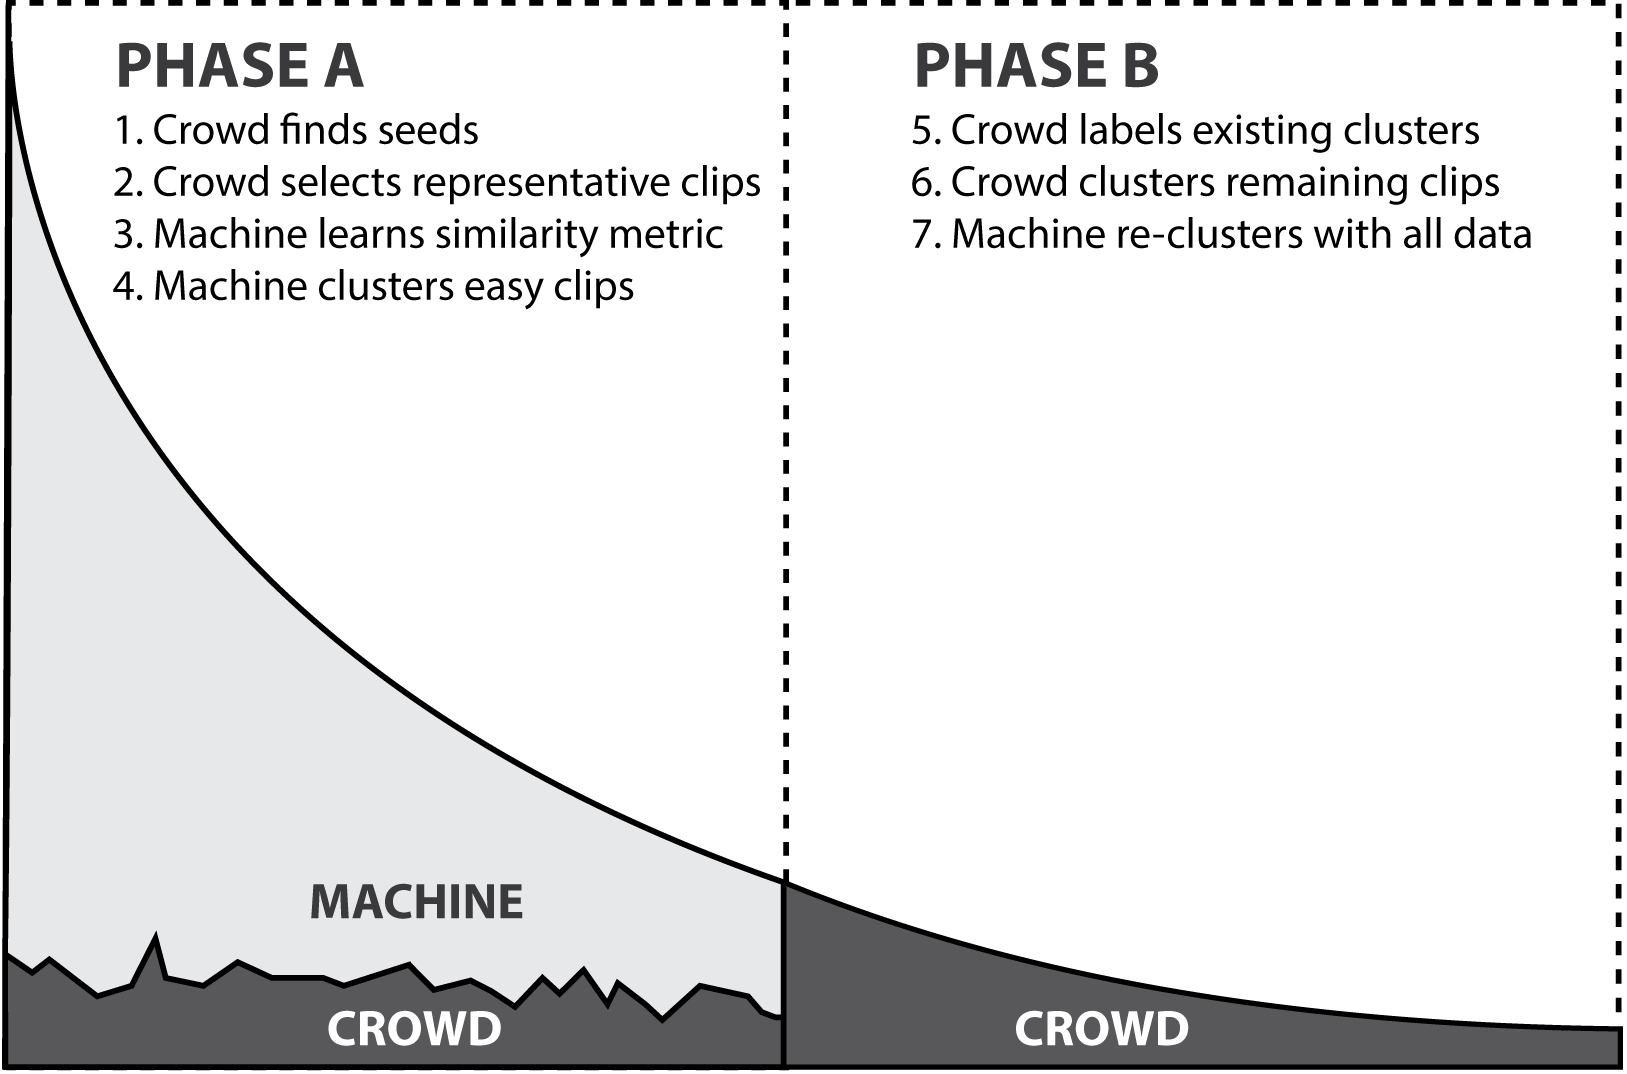
\includegraphics[width=0.6\columnwidth]{Chapters/Alloy/images/alloy_overview_01.png}
%	\caption{First, we use the crowd for creating labels and select features to
%		train a machine learning model. Then, the trained model clusters a
%		large part of the input data.  Finally, the crowd takesover again to
%		refine the output from the machine to produce the final result.}
	\caption[A conceptual overview of the Alloy system.]{
		A conceptual overview of the system. In the first phase, crowd workers identify
		seed clips to train a machine learning model, which is used to classify
		the ``head'' of the distribution. In the second phase, crowd workers classify
		the more difficult items in the ``tail''. A machine learning backbone provides
		a consistent way to connect worker judgments in different phases.
	}
	\label{fig:workflow}
\end{figure}

% - Clustering unstructured information is important, but current machine algorithms have problems understanding deeper semantics of rich textual data. 
% - Recent research has begun to ..., <give examples of current work's success> However, <move examples from related work>.

Clustering, or pulling out the patterns or themes among documents, is a fundamental way of organizing information and is widely applicable to contexts ranging from web search (clustering pages) to academic research (clustering articles) to consumer decision making (clustering product reviews) \cite{jain1999data}.  
For example, a researcher may try to pull out the key research topics in a field for a literature review, or a Wikipedia editor may try to understand the common topics of discussion about a page in order to avoid or address previous conflicts. Doing so involves complex cognitive processing requiring an understanding of how concepts are related to each other and learning the meaningful differences among them \cite{Bellman:2003:DP:862270,kriegel2009clustering,medin1978context}. 

Computational tools such as machine learning have made great strides in automating the clustering process \cite{blei2003latent,chuang2012termite,chaney2012visualizing}. However, a lack of semantic understanding to recognize the important differences between clusters leaves the difficult task of identifying meaningful concepts to the human analyst \cite{chuang2012interpretation}. This reflects an inherent advantage for humans over machines for the complex problem of understanding unstructured data beyond merely measuring surface similarity, and a corresponding opportunity for research in combining human and computational judgments to process complex information \cite{fails2003interactive, Kulesza:2014:SLF:2611247.2557238, hu2014interactive}.

One such promising avenue of research harnesses the power of crowds to identify categories and cluster rich textual data. Crowdsourcing approaches such as Cascade, Deluge, and Crowd Synthesis \cite{chilton2013cascade,bragg2013crowdsourcing,andre2014crowd} have demonstrated the power of splitting up rich, complex datasets into small chunks which can be distributed across many human coders. However, all of these approaches must grapple with a fundamental problem: since each human coder is seeing only a small part of the whole dataset, a lack of global context can lead to incoherent results.  For example, if the items sampled are too similar, the worker might create overly fine-grained clusters. On the other hand, if the items sampled are too dissimilar, the worker might create overly broad clusters. Clusters found in many worker segmentation sets may give rise to redundant clusters, while clusters whose items are sparsely split among segmentation sets may never be realized at all. As an example, \cite{andre2014crowd} cite redundancies in Cascade's top level clusters having both ``green'' and ``seafoam green'', ``blue" and ``aqua'', as well as the encompassing category of ``pastels''. While Crowd Synthesis used an iterative approach to address these redundancy problems, it trades this off with lowered robustness as issues with early workers' categories can cascade throughout subsequent workers' judgments. This suggests the design space of approaches for crowd clustering may be being critically limited by the assumption of splitting up the dataset into small, fixed pieces that prevent workers from gaining a more global context.

Another challenge with current crowd clustering approaches is that using human judgments to label each piece of data is costly and inefficient. Deluge addresses some issues with efficiency, improving on Cascade by reducing the number of human judgments elicited as the rate of new category generation slows \cite{chilton2013cascade}. However, these crowd clustering algorithms still require human judgments for every item, which is costly. In the real world data often follows a long-tailed distribution in which much of the data is captured by a small number of categories in the head of the distribution \cite{white2007studying}. For such data in which many items in the head of the distribution are likely to be highly similar, once humans have identified the meaningful categories and representative examples it would be more efficient if a machine could classify the remaining items in those categories. A danger with such an approach is that the sparse categories in the tail of the distribution with few examples may be difficult to train a machine to recognize, and so human judgments may have another important role in ``cleaning up'' low frequency categories.

%Past work also explored ways to combine expert workers and computation for categorizing unstructured textual information using interactive interfaces \cite{huang2006text,settles2011closing}.
%Both studies showed that using one expert worker to identify a small set of informative keywords can significantly improve the results of machine clustering on the 20 newsgroup dataset, where each category has similar number of articles.
%However, it is also common for a collection of information to be not evenly distributed across topics, but instead follow a highly skewed distribution \cite{white2007studying}. In such cases, statistical based algorithms may perform well on the typical cases in prominent topics of the dataset, but fail to capture the edge cases and the smaller categories. 
%Intuitively, it could be greatly beneficial to use human judgements again to clean up the output, covering cases that are difficult for the machines but relatively simple for people.


%Such advantage is partly based on a good global understanding of the information at hand, which either comes from prior knowledge and/or comprehending the entire dataset for expert workers.
%However, this creates challenges for system designers due to the distributed nature of crowdsourcing \cite{Kittur:2013:FCW:2441776.2441923}, namely the lack of domain knowledge of the workers and the difficulty of providing enough global information in a microtask for finding good categories.
%Since it is infeasible to ask crowdworkers to read all items in the dataset, current work simply employs crowdworkers to process arbitrarily parts of the dataset \cite{chilton2013cascade,andre2014crowd}. 
%This lack of global context can lead to incoherent results, because different workers are creating clusters based on different small pieces of the puzzle. For example, if the items sampled are too similar, the worker might create overly fine-grained clusters. On the other hand, if the items sampled are too dissimilar, the worker might create overly broad clusters. 
%In general, most current systems provide context by showing a small sample of items, hoping that it captures the distribution of information in the larger dataset. 

%People have been developing machine learning algorithms to cluster unstructured rich textual data using similarity measurements based on surface features. However, without deeper semantic understanding of the information at hand, it can be difficult for machines to distinguish which features embody useful categories.
% For example, \emph{sunlight} and \emph{lights} are potentially good features for the first text clip in Figure~3 if other items in the dataset are about ways to better grow tomatoes, but not so if other items are about the seeding of various plants. 
%For example, \emph{liquid water} is potentially a good feature for the second text clip in Figure~3 if other items in the dataset are about key factors of supporting life on a planet, but not so if other items are about the various roadmaps of NASA. 
%Human intellect, on the other hand, is readily able to infer meaningful categories from complex data given enough context  \cite{Bellman:2003:DP:862270,kriegel2009clustering,medin1978context}. This gives crowds an inherent advantage over machines for the complex problem of understanding unstructured data beyond merely measuring surface similarities, and a corresponding opportunity for research in combining crowds and computation to cluster complex information.



% 
% \joseph{new}
% % moded from the info-seeking framing
% Whether researchers, shoppers, students, or voters, a common challenge is
% synthesizing information gathered from multiple sources into
% meaningful and useful categories
% to gain a bigger picture in order to 
% identify the core topics,
% such as specs for a new product, ways to
% unclog a drain, organizing research papers into conference session, or the key issues
% involved in an election. 
% For example, an individual searching for health information may have
% to go to over a dozen web sites in order to get a complete picture of a domain
% \cite{bhavnani2005difficult}. While doing so information seekers aim to
% determine the common themes and the distribution of information across those
% themes, eventually trying to decide which information is important and which sources to
% trust \cite{kittur2014standing}.  This represents a substantial cognitive
% challenge and a corresponding opportunity for research in better supporting
% individuals engaged in these tasks. 

% dont draw attention to scaling
%In this paper, we explore an alternative approach of an ad hoc, crowd-driven
%method for finding structures and organizing %datasets with less than a few thousand items.



% 1. keywords can help machines get much better results
% 2. skew distribution
% 3. machines output still needs human clean up 




% A key difference from previous work on crowd clustering is our two-stage model
% of clustering.
% %There is a conflict between providing sufficient context
% %for identifying categories in a skewed distribution and the limited context capacity of
% %microtasks that are suitable for posting to online crowdsourcing marketplaces such as Amazon Mechanical Turk. Further, i

% In such cases the head of the topic distribution
% contains a disproportionate number of clips, and once a human has labeled a few
% of these clips it is inefficient to continue using human labor to finish
% labeling them as automated methods can do a reasonably good job.  Conversely,
% the tail of the topic distribution contains topics with few clips,
% and expending resources to train a machine learning algorithm to
% identify these sparse topics is less advantageous, while it is comparatively
% easy for humans to classify these clips.

% Previous crowdsourcing research has shown success in using the crowds to capture uncommon cases in a long tailed distribution to improve inline answers in Web search engines \cite{Bernstein:2012:DAS:2207676.2207710}.



% 
% , it can lead to problems
% enforcing global constraints such as redundant or overly similar
% categories, categories at the wrong level of abstraction due to lack
% of context, categories that do not represent the distribution of
% information faithfully because of sampling issues, or simply inadequate categories
% because of worker motivation or expertise issues. 
%
% dont draw attention to scaling
% Furthermore, hiring workers
% incurs monetary costs and thus can have issues scaling to large amounts
% of data compared to computational approaches. 
%
% old framing for "the but"
% Existing crowd clustering approaches have addressed some of these
% challenges, but often with significant trade-offs. For example, 
% methods that are robust against a few poor judgements often fail to enforce global
% constraints, leading to overlapping, incoherent, or duplicated categories. On the other hand,
% methods that focus on producing
% coherent results by providing global view to the crowds are often vulnerable to a few
% poor judgements in early stages cascading through the workflow
% \cite{chilton2013cascade,andre2014crowd}.
%
% 
% This paper describes Alloy, a crowd-based short text clustering workflow that uses a \emph{sample-and-search} process to build up workers’ mental models with context beyond showing multiple arbitrary items.
% We believe this is a new way to support global context for crowd clustering.

% In addition, we introduce a \emph{cast-and-gather} framework that allows Alloy to cast out various types of microtasks for different types of human judgements, and gathers them using a machine learning backbone. With this framework, Alloy 
% incrementally cluster the datasets in a two-phase approach: First, workers actively request for context by repeatedly sampling random items and searching for similar items in the entire dataset while building up their mental model of the global context. Based their labels, a machine classifier then clusters unlabeled items with high confidence, capturing the prominent categories (the head of the distribution). Then, crowdworkers switch roles from trainers to cleaners, capturing smaller clusters and items that are difficult for the machine classifier (the tail of the distribution).

This chapter describes Alloy, a hybrid approach to text clustering that combines the richness of human semantic judgments with the power of machine algorithms. Alloy improves on previous crowd clustering approaches in two ways. First, it supports better global context through a new ``\emph{sample and search}'' crowd pattern which changes the crowd's task from classifying a fixed subset of items to actively sampling and querying the entire dataset. Second, it improves efficiency using initial crowd judgments to help a machine learning algorithm cluster high-confidence unlabeled items in the head of the distribution (prominent categories), and then uses later crowd judgments to improve the quality of machine clustering by covering the tail of the distribution (edge cases and smaller categories). 
To achieve these benefits, Alloy introduces a novel modular approach we call ``\emph{cast and gather}'' which employs a machine learning backbone to stitch together different types of crowd judgment tasks. While we provide a particular instantiation of the cast and gather approach here (with a hierarchical clustering backbone which gathers three types of crowd tasks, or ``casts''), the general framework for modularizing multiple types of human judgments with a common machine-based backbone may inspire application to other contexts as well.


% old framing for the therefore
% 
% We introduce Alloy,
% a new approach to structure complex information by identifying meaningful clusters of short text
% with crowds and computation.
% Alloy is based on the intuition that we
% can employ the crowd to act first as a guide, highlighting the high-level
% structure of a domain as training for a machine learning model; then, after
% the algorithm has classified instances that are easy for it to
% categorize, the crowd can further clean up the results by categorizing the
% remaining instances that proved more difficult. Different from many of the previous
% approaches which gather small and independent human judgements for all
% instances and stitch them together to infer concepts,
% we use a machine learning model to scale crowd judgements to cover unlabeled instances.  
% By using a two phase approach, we try to compensate for the shortcomings of crowdsourcing (e.g., lack of context,noise) and machine learning (e.g., sparse data, lack of semantic understanding) by utilizing techniques from both fields. 
% We focus on providing rich context
% to crowdworkers and transferring context between workers in different phases with a machine backbone algorithm.
% Using this approach we aim to enforce global constraints while
% also leveraging machine learning to increase scalability and to protect against
% poor worker input.

\subsection{Related Work}

%\niki{want to start with a paragraph that sets up the importance of clustering
%    itself and gets to the crowd framing faster. Like the paragraph two down
%    from here. I'd put these two paragraphs later in the intro or in a related
%    work section. Remember that an AC will probably skim the first couple
%    paragraphs to decide who to recruit as reviewers. }

Document and short text classification are well researched topics in natural
language processing and machine learning. With enough labeled training data,
state-of-the-art algorithms can often produce good results that are useful
in real world applications. Yet building such systems often requires expert
analysis of specific datasets both to manually design an organization scheme and
to manually label a large set of documents as training data. Unsupervised approaches, 
or clustering,
aim to discover structures on-demand and without expert preparation
\cite{jain1988algorithms,hartigan1975clustering,steinbach2000comparison}.
While these
data mining approaches may discover dimensions (features) that provide a good
separation of the dataset, the inferred categories can be difficult for a human
to interpret, and many of them may not capture the most meaningful or useful
structure in a domain due to high dimensionality or sparseness in the word vector space 
\cite{Bellman:2003:DP:862270,kriegel2009clustering}.
To deal with these issues, researchers have explored ways to automatically
discover topical keywords that can help identify useful categories in unstructured data
such as TF-IDF, latent semanic analysis, and latent
Dirichlet allocation \cite{manning2008introduction,Jones72astatistical,deerwester1990indexing,blei2003latent}.
However, even with these improvements, automatic methods often still
perform poorly, especially when the number of document is small, the lengths
of the documents are short, or when the information is sparse.


% 
% People have been utilizing different machine algorithms to organize 
% huge datasets
% such as research paper archives or newsgroup articles. Unsupervised methods, such as
% Latent Dirichlet Allocation \cite{blei2003latent}, rely on tens of thousands of articles for discovering
% salient features. However, there are also many cases where the amount of
% information at hand is less than sufficient for such methods. For example, during online exploratory 
% information seeking, people typically go through dozens of sources.
% When organizing sessions for a conference, there are typically a few hundred
% accepted papers. On the other hand, supervised methods
% can organize datasets of different scales once a classifier is trained,
% but it requires prior expert knowledge
% to define classes, precompile a large dataset, and create labels 
% for training. This process, besides being expensive in time and expertise, can also be
% difficult to adapt to a different context. For example, the classes designed for a CHI paper
% classifier may not be fine-grained enough to organize papers in a more focused conference
% such as CSCW. 



More recently, researchers have begun to use crowds to organize datasets without predefined categories.
Cascade \cite{chilton2013cascade}
attempts to address abstraction and sampling problems by first having
multiple workers generate categories for each item and then later having
workers choose between them. By providing limited context to each worker (8 items or 1 item with 5 categories), it suffers from 
categories that can have varying levels of specificity. As a follow up study, Deluge \cite{bragg2013crowdsourcing} produces
comparable results, but with significantly lower cost by optimizing
its workflow using machine algorithms. In another line of research, Crowd Synthesis \cite{andre2014crowd} showed that providing more context by simply showing more items can lead to significant better categories, suggesting that global context is one of the key elements for crowd clustering algorithms.
In general, most current systems provide context by showing a small sample of items, hoping that they captures the distribution of information in the larger dataset. 
We propose an alternative approach that builds up workers' mental models by asking them to repeatedly sample for new items, identify discriminative keywords, and search the dataset for similar items, taking advantage of people's capacity of information foraging \cite{pirolli1999information}.

% Furthermore, a dataset can be organized with very
% different categories for different purposes (e.g., author perspectives vs
% topics), and it is often difficult for unsupervised methods to
% take into account the context for organizing documents into conceptual groups.
% For these reasons, there seem to be room for exploring methods that make use of 
% both the crowd and machine to not just label documents with predefined classes
% for training supervised models, but also to identify the innate structure of
% the dataset that fits a given context.


% the info-seeking framing
% Whether researchers, shoppers, students, or voters, a common challenge is
% synthesizing information encountered from diverse online sources into
% meaningful and useful categories, such as specs for a new product, ways to
% unclog a drain, the factors that make a planet habitable, or the key issues
% involved in an election. Important information can be scattered across many
% sources; for example, an individual searching for health information may have
% to go to over a dozen web sites in order to get a complete picture of a domain
% \cite{bhavnani2005difficult}. While doing so information seekers aim to
% determine the common themes and the distribution of information across those
% themes, eventually trying to decide which information is important and which sources to
% trust \cite{kittur2014standing}.  This represents a substantial cognitive
% challenge and a corresponding opportunity for research in better supporting
% individuals engaged in these tasks. To provide a sense of the the magnitude of
% this opportunity, estimates put the amount of time spent on such complex
% sensemaking tasks at around 70 billion hours per year in the U.S. alone, or
% around 30\% of the time people spend online
% \cite{kellar2007field,Fisher:2012:DSI:2207676.2207711}.


A complementary set of approaches to crowd clustering research has focused on
addressing the scaling problem through computation, applying approaches such as
partial clustering \cite{yi2012crowdclustering}, learning similarity metrics
through triad-wise comparisons \cite{tamuz2011adaptively}, or using matrix
completion to reduce the number of labels needed from
workers \cite{yi2012semi}. 
While these approaches have shown to be powerful on simple
information such as images or travel tips, synthesizing more complex
information can be difficult without providing novice crowdworkers with richer
context or opportunities to deeply process the data. 

%
% Novices are especially
% susceptible to creating superficial categories, using too much or too little
% abstraction, or failing to notice a category entirely
% \cite{chilton2013cascade,andre2014crowd}.


% (remove b/c space)
% Some of the core challenges this approach addresses include:
% 
% \begin{itemize}
% \item \emph{Lack of expertise}. Typical crowdworkers do not have the domain expertise.
% 	Without enough context to help them build some background knowledge, they
% 	may cluster the data into superficial classes based on the surface patterns
% 	rather than deeper understanding of the information.  Furthermore, without
% 	enough context to provide some idea of the information landscape, they may
% 	also create classes that are too general and ill-organized.
% \item \emph{Disagreement}. Crowdworkers may create different and conflicting
% 	feedback, because they understand the same dataset from different
% 	angles, thus creating clusters based on different features.
% 	Further, even if they are working from similar viewpoints, they
% 	may create clusters at different levels of abstraction.
% \item \emph{Capacity}. The two challenges above can potentially be ameliorated
% 	by providing more contextual information to the crowdworkers. However, it
% 	is difficult to provide a large amount of information to build up their
% 	mental model, while keeping the microtasks manageable. In our case, it
% 	would be unreasonable to present the workers with the complete raw corpus,
% 	due to the size of the datasets.
% \item \emph{Aggregation}. Due to the \emph{capacity} challenge, each worker may
% 	only be working on a portion of the dataset. However, unlike tasks that
% 	label independent items, e.g., classify an image, items in the clustering
% 	task are not independent.  If each crowd worker only worked on a small set
% 	of the data, how do we put their independent judgements together to form a
% 	complete answer?
% \end{itemize}

% Clustering data by analyzing the underlying structures to discover abstract
% themes and concepts is a common and important procedure in a wide variety of
% tasks ranging from human learning and decision making to market research and
% recommender systems. For example, grouping accepted papers to form conference
% sessions, segmenting markets to identify the target customers, and grouping
% similar product reviews to provide a quick overview.  Whether performed by a
% person or an algorithm, the essence of such processes involves identifying the
% salient features for a given context, recognizing similar items based on the
% identified features, and discovering abstract classes (concepts) to form
% clusters. The same dataset may also be clustered differently under different
% contexts. For example, libraries may organize books based on different topics,
% while online bookstores may organize their products based on the characteristic of
% their previous and potential buyers.  However, even for humans, this process
% can be time-consuming and cognitively taxing, because it requires a global view
% of the data and a deep understanding of the context and domain to determine the
% importance of different features and arrive at a coherent grouping of meaningful
% clusters.


% Researchers have also begun to explore the use of the crowd to discover partitions
% in different types of datasets. Earlier work focused on creating labeled
% datasets for supervised or semisupervised training
% \cite{Raykar:2010:LC:1756006.1859894} and clustering image datasets
% \cite{yi2012crowdclustering,tamuz2011adaptively}.  More recently, research
% efforts have also been made in clustering complex information represented in
% text  \cite{yi2012crowdclustering,andre2013community,andre2014crowd}.

% weak sauce
% Past work has dealt with general datasets that utilize crowdworkers' everyday
% knowledge (colors, general travel tips, images of everyday objects) or domain
% specific datasets (Wikipedia ``barnstar'' awards). Unlike previous approaches,
% we employ a multi-phase approach that accounts for the weaknesses of humans
% (e.g., scaling) and machines (e.g., understanding context). Specifically,  the
% crowd first learns the context of an information space, then provides feedback
% to train a machine learning algorithm for recognizing that same context. We then
% leverage the algorithm to classify many instances on the fly, and return to the
% crowd to verify and fix the machine's clustering.

% Niki's comment
% Why are we working with such clips?  I.e., why is it important to be able to
% cluster web clips? (e.g., 30\% of the time people spend online is about complex
% information seeking where people are trying to pull structure out of and
% synthesize pieces of information from across many web pages). Generally, I
% think this whole paragraph could be moved up to the beginning (right after your
% first paragraph) and used to frame the problem we are working on.  
% Niki's comment2
% we focus on the problem of clustering snippets of information from the web.
% This task is a critical part of a larger research program aiming to synthesize
% information from diverse web pages into a cohesive whole, and could help
% address the issue of information scatter on the web (Bhavnani cite).
% [actually, probably want to move this to later]

% that we can work on the same data but provide a new way of combining crowds
% and computation to make up for the weaknesses of each approach?
% ** how?
% Add a bridging sentence that gives the intuition of the approach.  E.g.,``The
% key idea is that we break the problem into two phases; in the first phase we
% use the crowd to train a machine classifier to cluster the majority of the
% dataset, and in the second phase we use the crowd to manually classify those
% data that were not easily clustered by the machine'' (or something like that)

% In this paper, we present an empirical study of a two-phase approach that makes
% use of both human computation and text processing algorithms to tackle the
% problem of clustering complex information.  The key idea is that we break the
% problem into two phases; first, we use the crowd to train a machine classifier
% to cluster the majority of the dataset, then, we use the crowd to manually
% classify those that were not easily clustered by the machine. More
% specifically, in Phase A, we partially cluster the input dataset at the level
% of abstraction that is based on the clustering agreement and feature (keywords)
% extraction from a number of crowdworkers collected via a partial clustering interface. A
% classifier is trained on-the-fly using the feedback from the crowdworkers to
% measure the pairwise similarity of the items in the dataset, and the
% agglomerative clustering algorithm is performed to create intermediate clusters
% that the majority workers agreed upon. In this phase, the workers only work
% with a portion of the entire dataset, but create feature dimensions that are
% applicable to all items in the datasets.  In Phase B, the partially clustered
% dataset from the previous phase is presented to a number of crowdworkers, and global
% clustering agreement is collected via a global clustering interface to form
% the final output. In this phase, the workers have access to the entire dataset,
% in which a large portion is already clustered. By using this two phase
% approach, the algorithm can effectively create clusters from complex datasets at
% appropriate level of abstraction, even for datasets that are too large to be presented
% in full to a single crowdworker.

% Major contributions of this work include:
% \begin{enumerate}
% 	\item We explore the possibility of using novice crowdworkers not only to
% 		create answer labels, but also to extract meaningful feature
% 		dimensions through an interactive search process and train an SVM model
% 		to measure the similarity between items.
% 	\item We propose a method that is robust even if a few workers provided
% 		poorly organized results. Where as in previous systems, a single
% 		crowdworker labeling every item with a general topic (e.g.,
% 		\emph{solutions} or \emph{tips}) can have devistating effects on the
% 		quality of the feedback from subsequent crowdworkers.
% 	\item We use a two-phase process that makes use of both statistical models
% 		and aggregates agreements among crowdworkers to produce clusters at an
% 		appropriate level of abstraction for the given context.
% 	\item Previous work are mostly evaluated on clean datasets, where all items
% 		are valid, while we work with noisy datasets of short webclips gathered
% 		by crowdworkers, showing how the process can be robust to even 30\% bad
% 		input.
% % Niki: Why is this a contribution?  Maybe because we are sharing the gold standard data?
% % 	\item In addition to reviewing the clustering results for evaluation, we
% % 		created gold standard answers for complex datasets. We also present
% % 		inter-annotator agreements for each collections, and discuss the innate
% % 		properties of each corpus and how they effect the clustering process.
% \end{enumerate}


% ^^^^^ FINAL ANSWER AREA ^^^^^

% The rest of the paper is organized as follows: In the next section, we review
% previous works that are most relevant to our research. We then describe in
% detail the two-phase produces of the proposed method in the Method Section. We
% also explain the experimental settings and the datasets.  Finally, we show the
% empirical results of our experiments, and conclude in the last section.




% \section{Related Work}
% %!TEX root = main.tex

There have been a variety of methods proposed in the literature, which differ
in many ways from ours.
%Make this a little bit more like an introduction than a lame phrase

\subsection{Word Sense Disambiguation}

Because human languages can be fuzzy and ambiguous, their exists a large amount 
of uncertainty around the meaning of a particular word when processing it. Word sense 
disambiguation (WSD), an open problem in natural language processing, attempts to solve
this by mapping ambiguous words to their intended concepts.  In 1995, Yarowsky proposed a novel
unsupervised WSD algorithm that rivals state-of-the-art supervised algorithms
\cite{yarowsky1995unsupervised}. The algorithm was based on the hypothesis of
``one sense per collocation'', which suggests a member of a set of keywords in
context is often sufficient to determine the sense of the nearby target word.
For example, the two sets of keywords for the word ``\emph{plants}'' are
``\emph{growth}, \emph{height}, \emph{flower}, \emph{fruit}, \emph{space}''
(for the \emph{life} sense) and ``\emph{car}, \emph{union}, \emph{equipment},
\emph{assembly}, \emph{nuclear}, \emph{job}'' (for the \emph{manufacturing}
sense).  Other research has suggested that when clustering documents using
topics or concepts, %a little confused about this word use%
a few informative keywords can yield good results
\cite{huang2006text}. More recent research has begun to explore the
possibility of representing words as contextual vectors
\cite{mikolov2013linguistic}, and represent short texts using distributional
semantic vectors \cite{socher2012semantic,socher2013recursive}. We designed our
method based on these observations, and used the crowd to identify important
keywords from the clips to improve clustering performance.


\subsection{Topic Modeling and Latent Semantic Analysis}

% move citations for LDA / LSA to settings and/or eval

In natural language processing, topic modeling is the process of using
unsupervised statistical models to discover abstract topics from a large set of
documents. In particular, Latent Dirichlet Allocation (LDA)
\cite{blei2003latent} is a widely used generative model under which each
document is generated with multiple topics, and each topic is a probability
distribution of words.  It is difficult for topic models to perform well for
collections of short text, since LDA relies on counting words in the documents
as probability distributions to discover topics.  In our work, we focus on
organizing small web clips that typically have a single topic, contradicting
the assumptions of the LDA generative model. On the other hand, latent semantic
analysis (LSA) ( Cite) seems more suitable for our gaol. It reduces word vector
dimensions by grouping words together to form concept dimensions based on their
occurrence in similar documents.

To compare the proposed method against these natural language techniques, we
also clustered the dataset using LSA and LDA as baseline systems in our
evaluation.

\subsection{Clustering High-dimensional Text Data}

With the high dimensionality of the word vector space, the distance, or
similarity, between two documents is diluted and hence unreliable. Additionally,
different ways of clustering the corpus may exist in multiple different
subspaces, i.e., using a subset of all dimensions, and most of them could be meaningless for the given context %hmmm, explain subspaces a little more%
\cite{kriegel2009clustering}. Consider a collection of snippets about planets in
the Universe.  One trivial way of organizing this collection is to cluster
snippets according to the planetary systems involved.  However, many other ways
of clustering may also make sense, such as the mass of the planets, the
temperature of the planet, or even the writing styles of the clips or the
number of typos in the clips.

People, on the other hand, seem to be capable of organizing documents into
clusters appropriately.  Given enough background information, people are
generally good at identifying the key idea of the documents, and create
clusters that are appropriate for the given context \cite{medin1978context}. In
our work, we employ crowdworkers to cluster
complex textual data, utilizing different techniques to provide them with background
information while they perform the task. 

\subsection{Clustering based on Human Computation}

Research efforts have also focused on the application of human computation 
to address the issues with machine only approaches. Two major approaches have
been taken to make use of human computation to improve clustering and 
classification of complex data. %hmm this is a bit of a weak paragraph %

The first approach focuses on using crowdworkers to label training data for
machine learning models, rather than relying on domain experts. 
Approaches related to this category includes creating labeled dataset
using the crowd \cite{snow2008cheap}, crowd base evaluation
\cite{callison2009fast}, and extracting accurate labels based on redundancy
\cite{ipeirotis2010quality}. We took a similar approach for the first part of
the system by using crowdworkers to not only help us create labels
for training an machine learning model, but to also extract salient words as features.

The second approach focuses on designing a crowd workflow that breaks down the
clustering problem into microtasks for novice crowdworkers, and combining the
results to form a complete answer.  Chilton et al. explored using the crowd to
create hierarchical clusters of concepts represented in short snippets of text
\cite{chilton2013cascade}. The task is broken down into three microtasks:
Generate, SelectBest, and Categorize. These microtasks focus on creating
semantic descriptions for clusters, finding the abstraction levels of the
descriptions, and grouping clips into the clusters. The goal is to produce a
hierarchical structure of the dataset. The error rates in the hierarchical
structure are 13\% to 27\%.  In our case, we also rely on crowdworkers to
generate semantic descriptions for the clusters. However, instead of building a
hierarchical structure, we focus on finding coherent clusters at a similar
level of abstraction for the given context.
%This last phrase is also a little confusing, what do you mean by coherent level? J: changed to 'similar'%

To explore the design of microtasks for performing distributed clustering using
the crowd, Andr\'e et al. (2014) investigated different approaches to present
context to crowdworkers for clustering complex concepts represented in short
text \cite{andre2014crowd}. Empirical study shows that providing context by
presenting multiple items to each crowdworker leads to significant improvements
on precision, recall, and accuracy of concept description.  The reported
precision rates range from 40\% to 65\%, and recall from 35\% to 82\%. We adapt a
similar approach of presenting multiple items from the datasets to provide
context.  Furthermore, to provide even more context, we also allow the
crowdworkers to randomly sample clips from the dataset, and to search the
entire dataset using keywords.

Besides using the crowd to cluster complex information, researchers
have also investigated the timing for conducting clustering in the information foraging
process \cite{kittur2013costs}. Participants were asked to gather information
online, and create categories, attributes and values for the gathered
information.  They were split into groups, and asked to created structures at
different stages.  Empirical study shows that by eliciting structure after all
the information is gathered leads to better structured data, as oppose to
creating structures while gathering information, when the participants have not
yet developed richer mental models.  Therefore, we focus on organizing the
datasets after the gathering process, as oppose to during the gathering
process.

Huang and Mitchell proposed an interactive system for classifying emails
\cite{huang2006text}. The proposed method is an expectation maximization (EM)
algorithm that incorporates the contents of the documents and also user
feedback. Similar to previous findings, they also assume that a few important
words may be sufficient to determine the category of the documents. The system
assumes a generative model in which each word in a documents is either
generated from one of the topic model of each category, or from a global
general topic. The user can provide feedback by associating keywords with a
category or associating a document with a category.  The feedback is
incorporated in the EM process as partially revealing the hidden values.
Different from our work, the system is designed for a single user to organize
their own documents, and to provide clustering results as suggestions based on
the user's preferences. We focus on using statistical models and designing
microtasks to employ the crowd to solve this problem.

Other approaches to crowd clustering have tried to address the scaling issues
by using computation, applying approaches such as partial clustering
\cite{yi2012crowdclustering}, learning similarity metrics through triad-wise
comparisons \cite{tamuz2011adaptively}, or using matrix completion
\cite{yi2012semi} to reduce the number of labels needed from workers. Unlike
these approaches, ours 1) deals with rich textual data and 2) uses a two-step
process. Crowds are used to first guide machines in learning how to
classify the data and then after the machine classifies what it can with high
probability, crowds are again used to ``clean up'' the data that is difficult
to classify.



\section{System Design}
%!TEX root = main.tex

% \nathan{I think you need to better define what you mean by "primitive". Its usage is a bit confusing}
% \jeffrz{Don't explain what you're going to present, just tell me what you did! Also, "method" is a weird heading.}

% In this section, we will present in detail the different human intelligent tasks (HITs)
% of three primitives, and the computations that drive them.  We will
% also describe a backbone algorithm that is used to flexibly connect different
% primitives to form a complete workflow.  In the Experiment Sections we will show
% the results of three workflows that consist of different combinations of these
% primitives.

The Alloy system clusters a collection of clips, or short text descriptions (Figure~\ref{fig:phase1-example}), using a machine learning backbone that gathers various judgments from human workers. In our terminology, each human task is a ``Cast'' for human judgements which are then ``Gathered'' together with the machine learning backbone. Alloy enables Casts (here, crowdworker tasks) of different types and in different orders to be fused together by calling a Gather after each one. In each Cast stages, arbitrary number of workers can be hired for better robustness or lower cost. In this chapter, we present three types of Casts with different purposes as well as one type of Gather. At a high level, the ``Head Cast'' is aimed at finding common categories in the head of the distribution, while the ``Tail Cast'' is aimed at classifying categories in the tail of the distribution for which machine clustering has low confidence. The ``Merge Cast'' aims to clean up existing categories by combining highly similar categories. We also describe a Gather Backbone that fuses the judgements from multiple crowdworkers,
and connects multiple casts to form complete workflows. For ease of exposition we introduce each component in the context of a typical workflow: the Head Cast, the Gather, the Merge Cast, and the Tail Cast.


% We will now describe in detail how we elicit different types of human judgements
% to iteratively organize different parts of a dataset. The Head Cast captures salient
% keywords to uncover prominent categories that covers the head of the distribution. The Merge Cast cleans up
% existing categories by
% identifying duplications and combining them to form coherent structures. Finally, 
% the Tail Cast cleans up the remaining clips and identifies small categories to cover the tail of the distribution.
% We will also describe a Gather Backbone that fuses the judgements from multiple crowdworkers,
% and connects multiple casts to form complete workflows.
% In the following subsections, we will introduce them in the general order of actual workflows:
% Head Cast, Gather Backbone, Merge Cast, and Tail Cast.


\begin{figure}
	\centering
	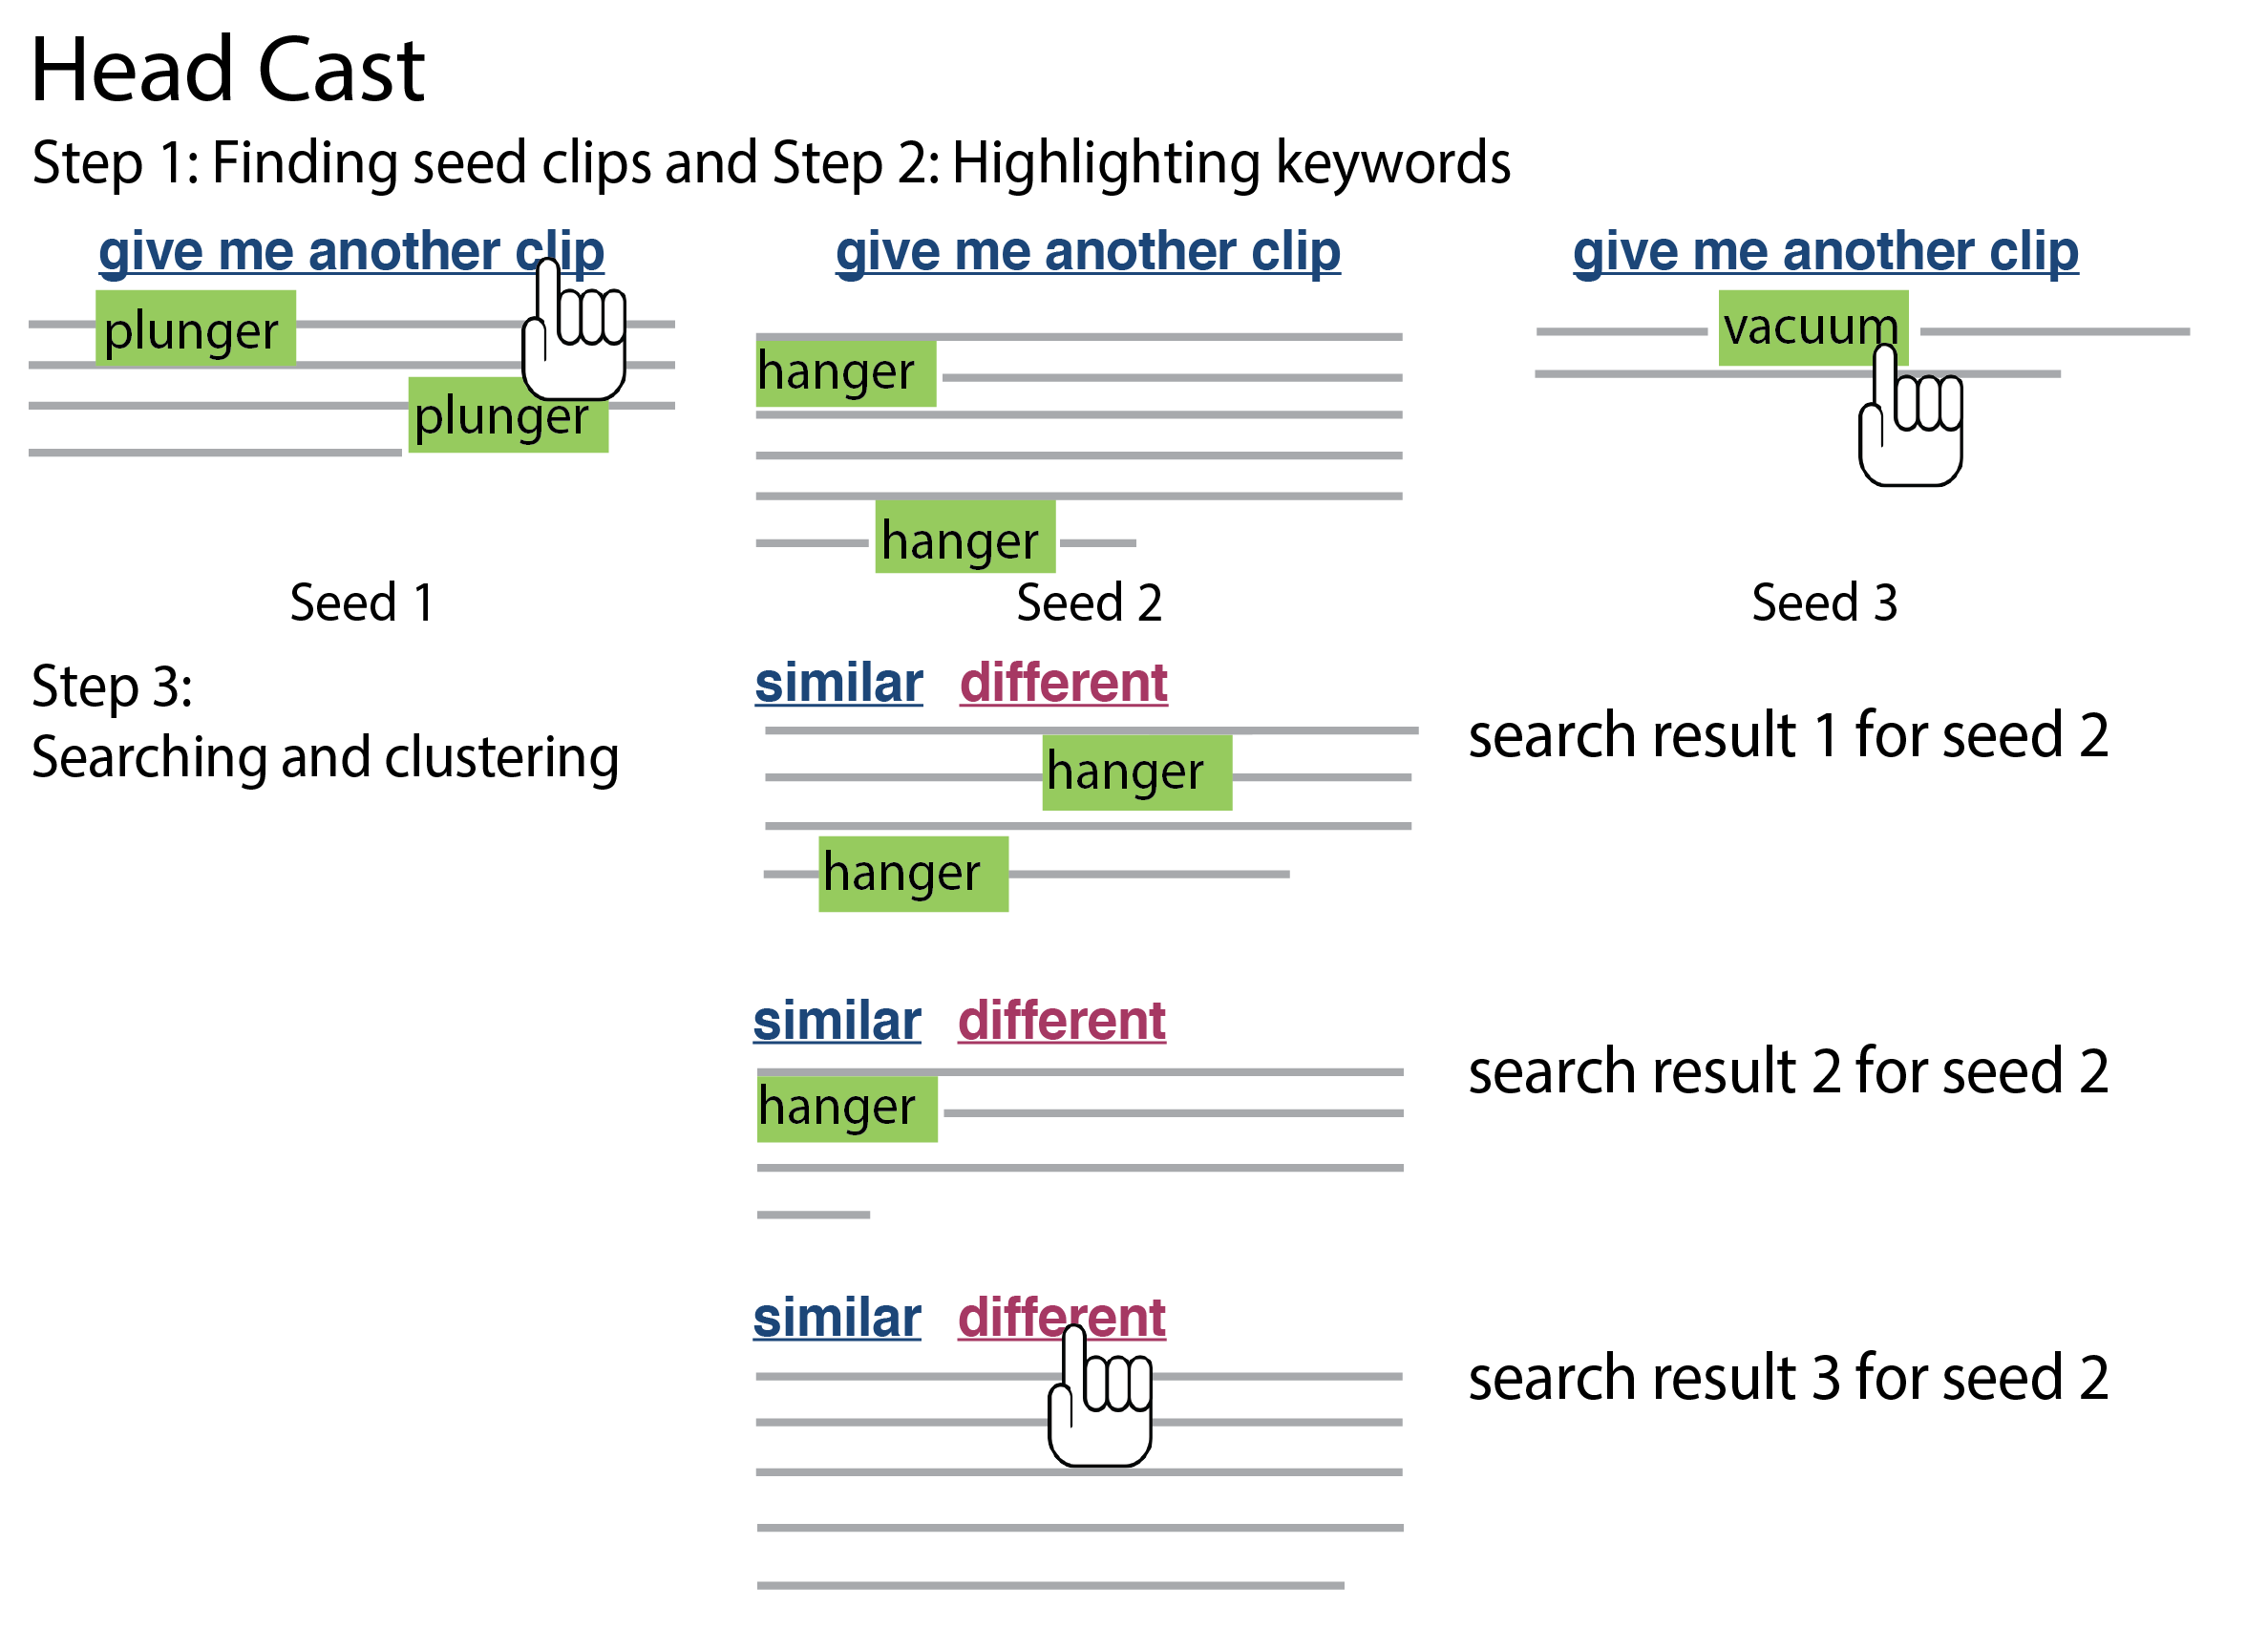
\includegraphics[width=0.6\columnwidth]{Chapters/Alloy/images/clusteringv2-04.png}
	\caption{The interface and steps of the Head Cast HIT.}
	\label{fig:phase1-hit}
\end{figure}

\subsection{The Head Cast}
The Head Cast aims to identify salient keywords to uncover the most common
categories in the head of the distribution. Doing so involves challenges in
providing workers sufficient context to know what a good category is, and also
in how to structure their work process in order to train a machine learning
algorithm to take over the classification of categories based on
human-identified seeds and keywords. 
Previous studies show that presenting multiple items from a collection can help
provide context to human workers \cite{medlin1978}, increasing the likelihood
of obtaining better clusters.  However, it can be difficult to determine how
much context is sufficient and how to produce a good sample that captures the
distribution of information of the whole dataset. 
Therefore, we introduce a new crowd-pattern we call ``\emph{sample and
    search}'' for providing global context through active sampling and
searching with keywords.   We ask crowdworkers to identify coherent categories
by presenting with four random items, but allowing them to replace each item by
random sampling from the entire dataset until they are confident that the items
will be in different categories in the final output.  This requirement gives them
the motivation to build up better global understanding of the dataset through
repeated sampling. After obtaining the four seed items, we ask crowdworkers to
identify keywords in each clips to search for related items in the dataset.
This process takes advantage of people's capacity of finding new information
\cite{pirolli1999information}. To create a familiar experience, we allow the
workers to freely change their query terms and update the search results in real
time. This way they can refine their searches based on the results, the same
way as when conducting online information foraging tasks \cite{jansen2009patterns}.
As shown in Figure~\ref{fig:phase1-hit}, the Head Cast HIT interface consists of three steps:

% The intuition is that a few keywords can be sufficient to
% identify important clusters in the head of the distribution
% \cite{huang2006text}. However, identifying important
% clusters and their salient words often requires a deep understanding of the
% data.

%The goal of Head Cast is to make use of human judgements to identify a set of
%keyword features and train an SVM model to partially cluster the given
%dataset \niki{this is a confusing way to introduce the SVM, since people will think you %are using it for clustering but you are using it more as a feature selection/similarity %metric enabler}.  Since it is infeasible to ask a crowdworker to organize the entire
%collection due to its size, each crowdworker
%worked on a small part of the dataset.  
% We implemented a three-stage workflow that uses machine learning models to augment initial human judgments.

%First, we use crowd workers to
%identify important topics and keywords through an interactive interface (Stage 1). Next we train an %SVM model to find the best set of features for predicting pairwise similarity of items based on the %human judgments (Stage
%2). Finally, we use those similarity judgments to create clusters using a
%hierarchical clustering backbone (Stage 3).

%\nathan{I changed the wording up here a bit}


% \jeffrz{***** If I were you, I'd make this two stages: stage 1 - human clustering, stage 2 - training and running an ML algorithm. this way you can echo the two-stage thing from the DESIGN section and reduce some redundancy}
% \joseph{two-phase actually refers to Head Cast and Tail Cast, not the steps here.}

% \subsubsection{Stage 1. Partial clustering and keyword extraction}

%Each crowdworker processes a
%portion of the input dataset using a set of four random seed clips we initially assign. 
%The idea is that most people are
%capable and familiar with picking out good keywords for retrieving documents
%through search. \nathan{maybe cite an IR paper about successful keyword search}.
%By asking crowdworkers to identify keywords in a seed clip to
%search for other clips that should be in the same category, we can record the
%process and gather not only clustering labels but also good feature dimensions
%at the same time.


\begin{enumerate}
    \setlength\itemsep{-1mm}

	\item \textbf{Finding seeds}:
    	Four random seed clips are presented to each crowdworker. Over each clip,
    	there is a button that allows them to replace the clip with another
    	random clip from the dataset.
		They are then asked to replace any clips
		that are too similar to the other seed clips.
		The workers repeatedly replace the seed clips
		until the four clips at hand belong to four different
		answer categories.
	\item \textbf{Highlighting keywords}:
	    The crowdworker is then instructed to highlight one to three
		unique keywords from each of the four seed clips that best identify
		their topics.  
	\item \textbf{Search and label}:
	    For each seed clip, we automatically search for
		similar clips from the entire corpus based on the highlighted keywords 
        and TF-IDF cosine similarity.
        The crowdworker is
		asked to label the top nine search results as \emph{similar} to or
		\emph{different} from their seed clips.
\end{enumerate}

% \niki{you need a rationale here; walk the reader through what problems you are solving with these steps so they can appreciate your solution.  Maybe reprupose stuff from the KA paper here, but you should adapt it so we don't get accused of plagiarism or something}

In Step 1, the crowdworkers need some understanding of the global context before
they can confidently judge that the seeds belong to different categories
in the final output. Previous work usually address this problem by presenting multiple
items to each crowdworker, in hopes of sampling both similar and dissimilar items
to give some sense of the global context. In reality it could be difficult to
judge how many items is sufficient for different datasets, and overly small size could lead to
bad samples that are unrepresentative of the global distribution.
We took a different approach by presenting fewer items at first,
but allowing workers to replace the seeds with random clips from
the dataset. This provide them both the mechanism and motivation to explore the dataset
until they have enough context to find good seed clips.

%The output of this stage is a number of potentially overlapping clusters, each
%contain one seed clip and nine other clips labeled as ``similar'' or
%``different''.

% unclear
%\begin{figure}[!h]
%	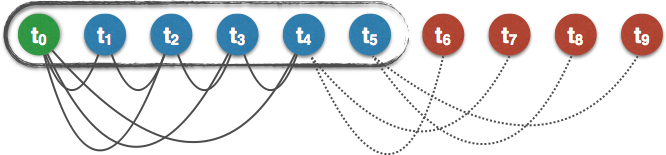
\includegraphics[width=0.9\columnwidth]{images/svm-clusters.png}
%	\caption{In Head Cast Stage1, crowdworkers create a cluster by selecting a
%		seed clip (green), and labeling 9 other clips as similar (blue) or
%		different (red). Each line connecting two clips indicates a training
%		events for Stage2.}
%	\label{fig:svm-clusters}
%\end{figure}

The intuition behind Step 2 is that people are already familiar with picking out good 
keywords for searching documents related to a concept via their online information
seeking experiences. In addition, requiring them to highlight unique keywords in the seeds
first, further ensures that they are familiar with the concepts in the seed clips, before
they search for similar items. In Step 3, the crowdworkers can still change and refine their
highlights from Step 2, and the system will refresh the search results in realtime. This
gives the crowdworkers both the motivation and mechanism to extract better keywords that lead
to better search results to label.
In Figure~\ref{fig:phase1-example}, we show two example clips from the datasets
collected using the two questions: \emph{How do I get my tomato plants to produce
more tomatoes?} and \emph{What does a planet need to support life?}
The highlighted words in each clips are the keywords selected by
one of the crowdworkers, showing that workers are finding useful words for classification.

%\niki{add rationale here about how this helps them in the next stage. you don't have to CALL it a design pattern since that's in KA, but give the intuition}

\begin{figure}
	\fbox{ \vbox{

		\ttfamily
        \scriptsize

% bad example
%		We had that problem too.  We snaked the bathroom tub, sink, \& stool so
%		many times.  The answer came to us when we had to replace the stool.
%		We found a \hilight{plumber} in the \hilight{yellow} \hilight{pages}.
%		Got some good recommendations.  They came and snaked the stack!  You
%		have to go on the roof for that.  If you can access the stack, rent as
%		big a plumber's snake as possible and to the job yourself.  Be sure to
%		ask the rental agency lots of questions, they want their equipment back
%		in good shape too. Be sure to clean the snaket (sic) off too.  That is
%		just plain common courtesy.  You will save lots of little tub snaking
%		jobs in the future
%
%		\rule{\columnwidth}{0.4pt}

		Tomato seedlings will need either strong, direct \hilight{sunlight} or
		14-18 hours under grow \hilight{lights}. Place the young plants only a
		couple of inches from florescent grow lights. Plant your tomatoes
		outside in the sunniest part of your vegetable plot.

		\rule{\columnwidth}{0.4pt}

        In its astrobiology roadmap, NASA has defined the principal
        habitability criteria as "extended regions of \hilight{liquid}
        \hilight{water}, conditions favourable for the assembly of complex
        organic molecules, and energy sources to sustain metabolism
	}}
	\caption{Example clips from two datasets with crowd keywords.}
	\label{fig:phase1-example}
\end{figure}


% \begin{figure}
% \footnotesize
% \hrule
% \vspace{2 pt}
% \textbf{Input:}\\
% \indent \ \ \ \ \ \ \ $S_{i,j}$: \ Sets of similar and different clips from Head Cast Stage 1\\
% \indent \ \ \ \ \ \ \ $K$: The set of all keywords from Head Cast Stage 1 \\
% \textbf{Output:} \\
% \indent \ \ \ \ \ \ \ \textit{Clusters}: Clusters of similar clips \\
% \indent \ \ \ \ \ \ \ \textit{Singletons}: Unclustered clips \\
% \textbf{Description:}
% \begin{algorithmic}[1]
% \STATE Let \textit{Sim} = \{$(t, t')$ $t, t' \in S_{i,j}$, $t, t'$ labaled "Similar"\}
% \STATE Let \textit{Diff} = \{$(t, t')$ $t$ labaled "Similar", $t'$ labaled "Different"\}
% \STATE \textbf{For} each $event_i \in$ \textit{Sim} $\cup$ \textit{Diff}:
%     \STATE \ \ \ \ \ \ Let $label_i$ = \textit{yes}, if $event_i \in$ \textit{Sim}, \textit{no} otherwise \\
%     \STATE \ \ \ \ \ \ Generate feature $feat_{i}$ based on $t, t', K$
% \STATE Train classifier \textit{M} using $label$, and $feat$
% \STATE \textit{Clusters}, \textit{Singletons} = HierchicalCluster($D$, $M$)
% \STATE \textbf{Return} \textit{Clusters}, \textit{Singletons}
% \end{algorithmic}
% \hrule
% \label{fig:phaseAstage2stage3}
% \caption{Pseudocode for Head Cast: Stages 2 and 3}
% \end{figure}

%\subsubsection{Stage 2. Similarity function: training an SVM model}

To learn a similarity function between clips, we use the crowd
labels and keywords to train a classifier that predict how likely two clips
to be labeled as similar.
Although the judgments from workers via the HIT interface about which clips go together provide valuable training information, we need to leverage these judgments to bootstrap similarity judgments for the clips that they did not label and to resolve potentially conflicting or partial category judgments. 
To do so we trained an SVM classifier in real-time to identify the set of keywords that are most indicative of categories and predict whether two clips in the dataset belonged to the same cluster.  
The training events
are all possible pairwise combinations of clips in the clusters obtained with the HIT interface,
which may include both positive (similar) and negative (different).
The feature dimensions are all the keywords highlighted by the
crowdworkers, and the value of each dimension is the product of
the number of times that keyword occurred in the two clips.
In general,  the keywords labeled by the crowdworkers contain little irrelevant information
compared to all words in the clips, but there could
still be some highlighted words that are not indicative of a category. For
example, one crowdworker worked on the dataset for ``\emph{How do I unclog my
	bathtub drain?}'' labeled ``\emph{use}'', ``\emph{a}'', and ``\emph{plunger}'' as
three keywords. Even though \emph{plunger} is a very
indicative feature for clustering this dataset, the first two highlighted words
seem too general to be useful. 
Using a linear kernel to
estimate the weights for the different dimensions (i.e., keywords) seems well suited for
our purpose \cite{chang2011libsvm, wu2004probability}.
Further, if the same keyword is used by different crowdworkers but lead to
very different labels, the linear SVM model will give lower weight to the corresponding dimention and
thus lower the effects of keywords that are less indicative of the categories.
We use LIBSVM which
implements a variant of Platt scaling to estimate probability 
\cite{lin2007note,platt1999probabilistic}. The overall intuition is that the SVM classifier is doing a form of feature selection, weighting those words in clips that could maximally distinguish clips amongst clusters. 
% \niki{I don't know if this is right, but you need to provide something like this as a rationale for each of your sections. Usually good to start with a problem you are trying to solve.}





% \jeffrz{do you need the rest of the stuff here? sounds too technical unless related work is important or reviewers complained last time}
% \joseph{this is from the reviewers last time (why is SVM needed / selected), i am shortening it by taking out the part with selecting bigram and trigrams.}
%This can potentially be solved by allowing turkers to extract
%bi-gram or tri-gram features from the clips, but it will also %increase interface
%complexity and decrease the coverage of the identified features %(e.g.,
%\emph{plunger} vs \emph{use a plunger}). On the other hand, a linear


In a preliminary experiment, we tested using all words in the clips as features to train
the SVM model. The intuition is machine algorithms might do a better job at identifying
keywords that can outperform keywords identified by crowdworkers. However, the results
show that using all words as features did not yield better results, and having much
higher feature dimensions increases the training time significantly.

%\subsubsection{Stage 3. Hierarchical clustering}
%\niki{is this actually the Gather stage? maybe integrate it into the bottom of the gather backbone section below?}

Finally, with the probability output of the SVM model 
as a similarity function between clips and a stopping threshold of $0.5$ probability,
we use a hierarchical clustering algorithm 
that serves as the Gather Backbone to capture head clusters. 

% We also tested different thresholds and found that 0.5 is the best performing condition overall. The output is a set of clustered and
% unclustered clips.

%\jeffrz{I have no idea what BACKBONE: HIERARCHICAL CLUSTERING means. make it more descriptive. (though I'd watch a movie titled that)}


\begin{figure}
	\centering
	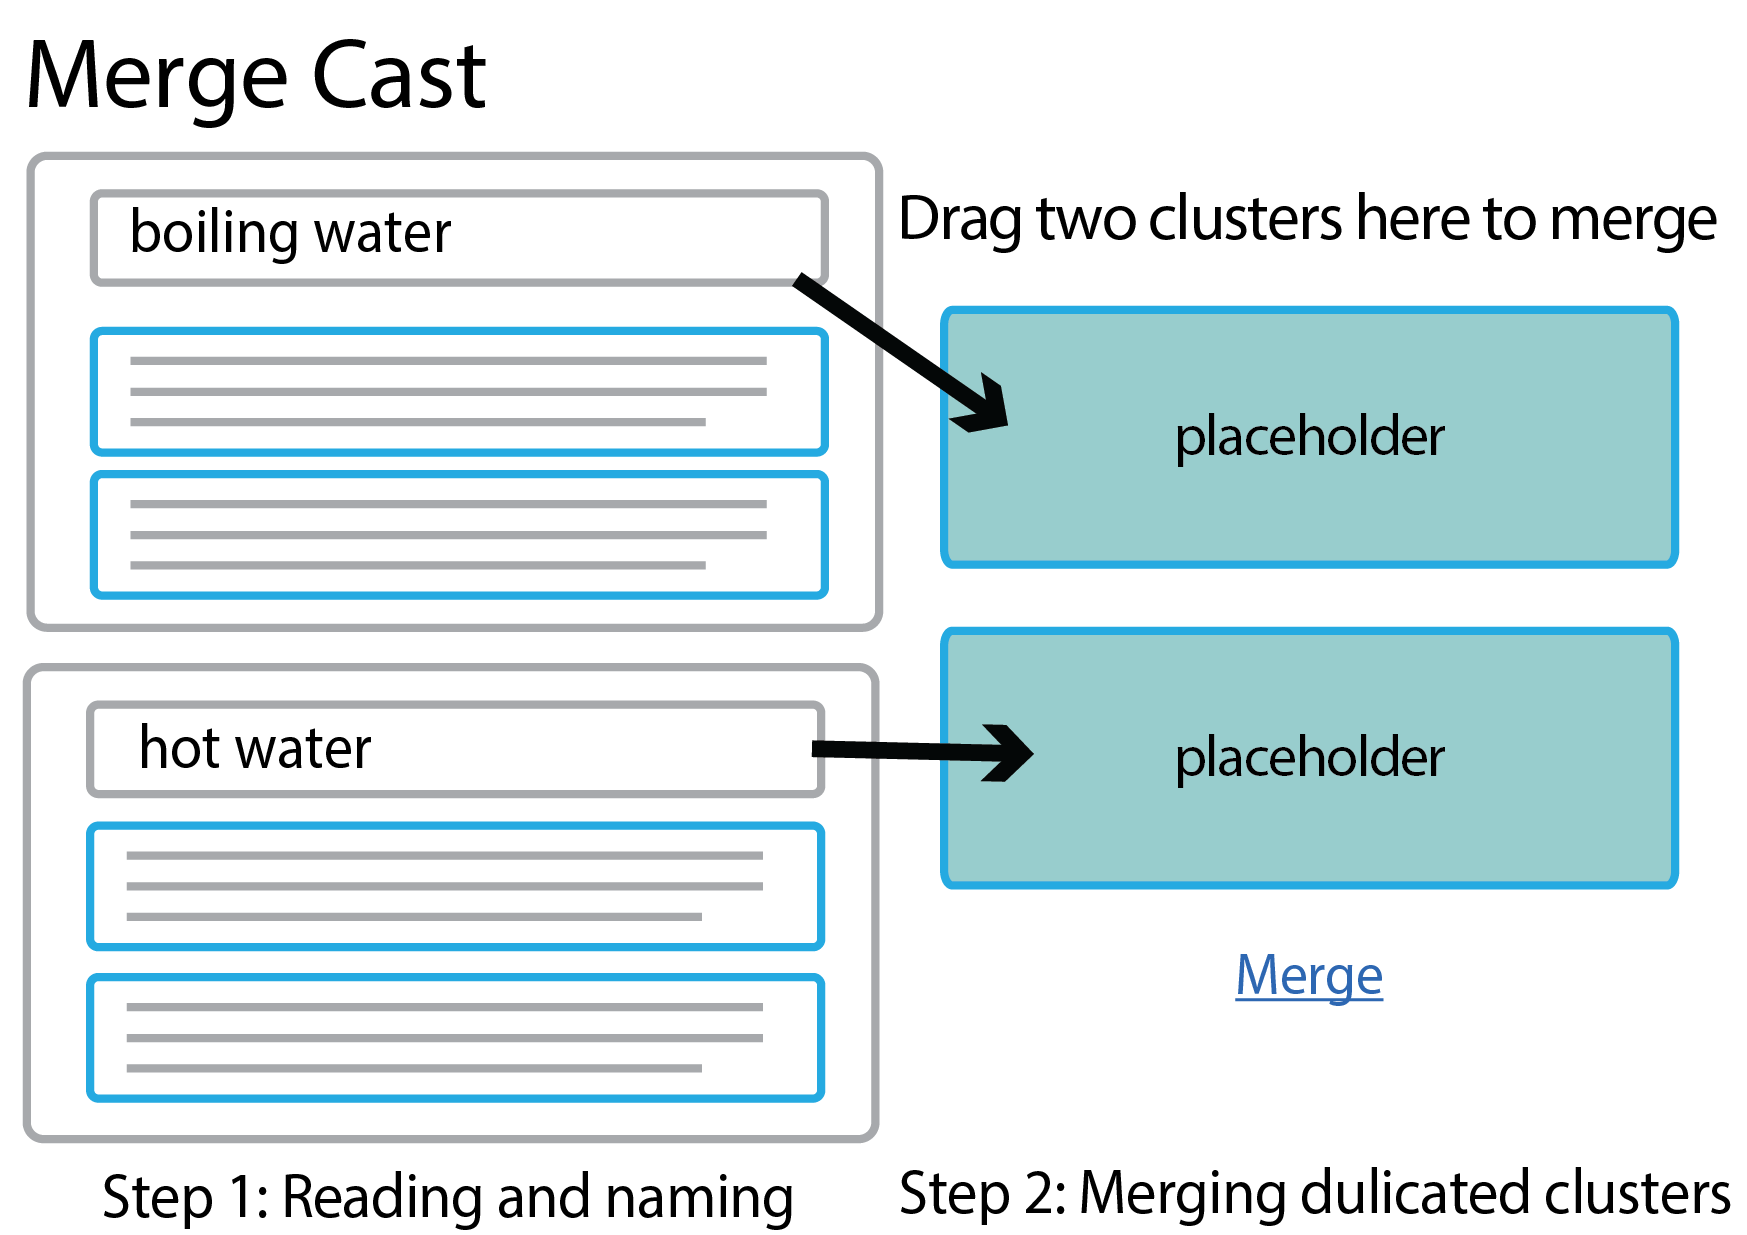
\includegraphics[width=0.47\columnwidth]{Chapters/Alloy/images/clusteringv2-02.png}
	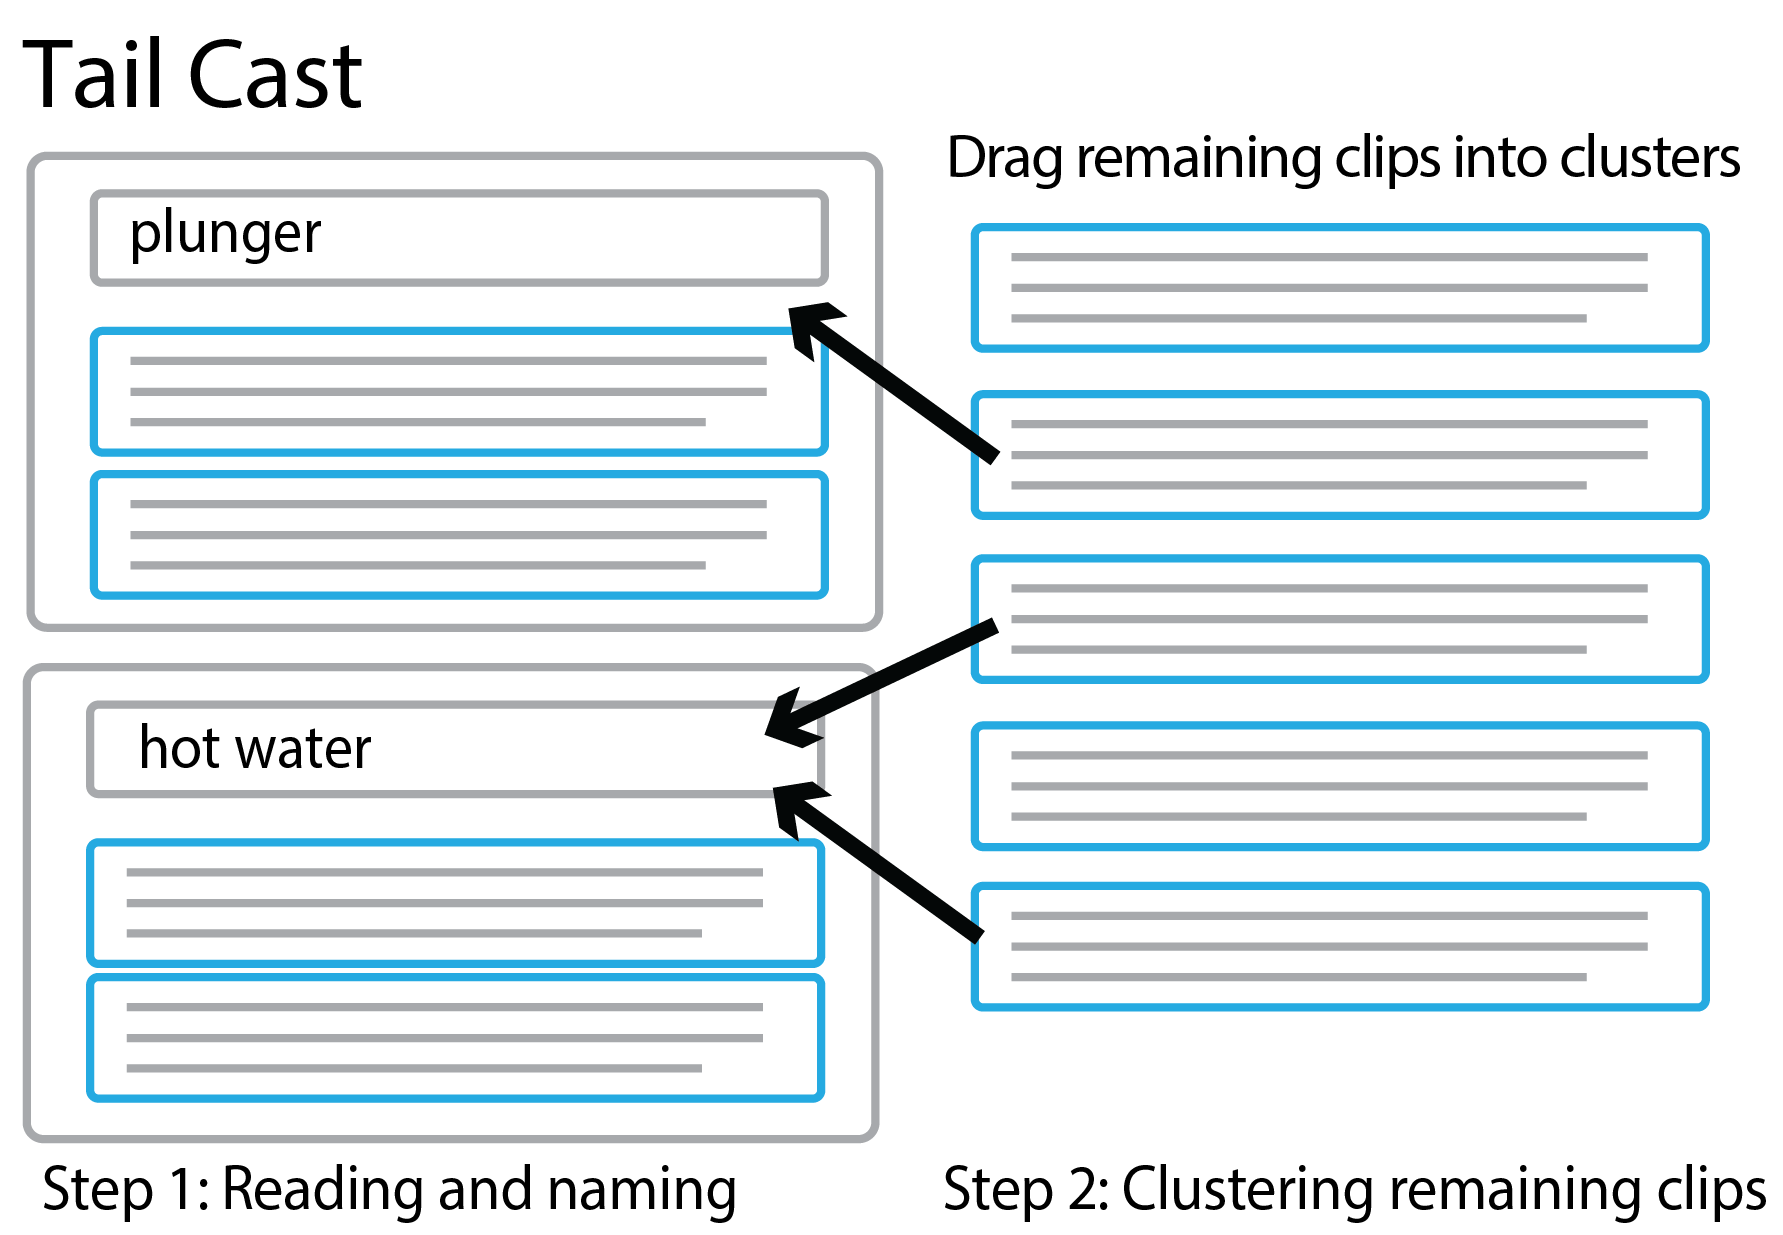
\includegraphics[width=0.47\columnwidth]{Chapters/Alloy/images/clusteringv2-03.png}
	\caption[HIT interface for the Merge Cast and the Tail Cast.]
        {The HITs for Merge Cast: Naming and merging existing
		clusters and Tail Cast: Clustering remaining clips.}
	\label{fig:phase2-hit}
\end{figure}

\subsection{Gather Backbone: Hierarchical Clustering}

\label{sec:hclustering}

%\jeffrz{I have no idea what primitives are now, and I am really, really lost. rewrite the two paragraphs as one}

Using a multiple-stage approach with different types of microtasks can make it
difficult to fuse together the different crowd judgements to form a coherent
result.  A key element to our approach in \textit{casting} for category
judgments in different ways is that we have a unifying mechanism to
\textit{gather} them back together.  For example, throughout our process we
cast for human category judgments in very different ways, including having
people identify seed clusters (the Head Cast), merge duplicated categories (the
Merge Cast), and classify the tail of the distribution (the Tail Cast).
Instead of creating ad-hoc links between these judgments we propose using a
unifying gathering mechanism composed of a machine learning backbone
which translates the different
\textit{casted} judgments into similarity strengths used as the basis of
clustering. We believe this \textit{Cast and Gather} pattern may be useful as
a way to conceptualize the relationship between machine algorithms and crowd
judgments for a variety of tasks.

% The Casts are designed to capture the varying types of human
% judgements that can be used to cluster different portions of the dataset. At
% different phases, the workflow iteratively creates new categories that cover
% more items in the dataset.

% remove candidate
To build a complete clustering workflow with multiple casts, we use a
hierarchical clustering algorithm as the backbone that connects different
casts. More specifically, the backbone algorithm  fuses the judgements
from different crowdworkers working on the same cast into
clusters, which, in turn, become the
shared context transferred to the next cast of the workflow.

With a clip similarity function from the prior cast and a stopping threshold, 
the hierarchical clustering method initially treats each clip as a
cluster by itself, and iteratively merges the two most similar clusters until a
threshold is reached. The result is a partially clustered dataset
with clusters and singletons. 
When the backbone is used after the last cast in the workflow, each
singleton is then merged into the most similar cluster.
The similarity between two clusters is defined as:

\vspace{-2mm}
\begin{equation}
	ClusterSim(\omega_1, \omega_2) = \frac{1}{|\omega_1||\omega_2|} \sum_{t_j \in \omega_1} \sum_{t_k \in \omega_2} ClipSim(t_j, t_k)
\end{equation}
\vspace{-1mm}

where $\omega_1$ and $\omega_2$ are the two clusters, $t_j$ and $t_k$ are each of the
clips in $\omega_1$ and $\omega_2$, respectively, and the $ClipSim()$ function is
the given similarity function between clips.


%\jeffrz{So we have Phase A, Consolidation Phase, and Phase B? I'm lost. Pick a "Phase" nomenclature and stick to it. I wouldn't do "Phase A", I'd give it a descriptive name kind of like you do here}
\subsection{The Merge Cast}
%\jeffrz{tighten this up. can you get by without "stages" and just paragraphs? you're losing lots of space on subheadings and nomenclature that may not be helpful unless it pops up again a few times in the paper}
%\niki{I would consistently go with "The Head Cast" instead of "Head Cast"}
While the Head Cast is designed to find the large clusters in the head of the
distribution, since each crowdworker works independently,
some of those clusters may actually
be different subsets of the same larger category or the same categories based
on different keywords (e.g., \emph{sunlight} vs \emph{natural lighting}).  The Merge Cast is designed to consolidate 
existing clusters by merging duplicated categories.  The input to this
cast is a set of clusters that may or may not cover the entire dataset,
and the output is fewer or equal number of clusters each with a list of ranked
short descriptions. 
The
challenge with detecting duplicate categories is that people need to understand
what is in each category first. 
We start by presenting a set of existing clusters, and asking crowdworkers to name 
each of them. This acts as a defensive design\cite{kittur2008crowdsourcing} that
ensures the crowdworkers
understand the current context (scope and abstraction level), and also to obtain
short descriptions for each of the clusters. 
Crowdworkers are
then asked to merge identical categories by dragging them into the
placeholders on the right (Figure~\ref{fig:phase2-hit}).

If there are too many head clusters to fit into a microtask,
the Merge Cast can be run recursively by
first running on disjoint sets of existing
clusters to consolidate them independently. Then, run another sets of
Merge Cast on the output of each initial Merge Casts, and recurse until
the output reduces to a set of clusters that
could be presented in a global Merge Cast to ensure consistency. 
The assumption here is that the set of clusters in the final output of Alloy should be
manageable by a single person to be useful.
We also wanted to point out that the number of clusters is likely to scale much slower than
the size of the dataset for many real-world data.
% In all six datasets we have tested, with up to 160 items, we have not encounter a case where we needed to run Merge Cast recursively.

% We can more formally characterize the scaling function as $T = log_c~N$,
% where $c$ represents the sparseness parameter of a dataset, $N$ the number of items 
% in the dataset, and $T$ the number of categories. The upper-bound limitation of 
% Alloy is then $T < L$, where $L$ is a limit on the complexity of a task given the characteristics of the 
% human computation platform utilized. Intuitively, this means that the Merge Cast will scale better 
% when the dataset involves fewer categories that explain more of the data, and when the human computation 
% platform supports more complex tasks.



With the labels from the crowdworkers,
we will again use the Gather Backbone to combine the judgements. The goal
is to merge existing clusters if more than half of the crowdworkers also
merged them in their solutions. Since in the Merge Cast
workers can not break up existing clusters or reassign clips, we can formulate 
the clip similarity function as:

\vspace{-2mm}
\begin{equation}
	ClipSim(t_1, t_2) = \frac{1}{N} |\{\omega: t_1, t_2 \in \omega \; and \; \omega \in \Omega\}|
\end{equation}
\vspace{-1mm}



where $t_1, t_2$ are the two clips, $N$ is the total number of crowdworkers,
$\Omega$ is the set of all clusters created by all crowdworkers, and $\omega$ is any cluster that contains both clips. This
function is robust against a few workers doing a
poor job. For example, if one crowdworker assigned every clip in the dataset to
a single, general cluster (e.g., \emph{answers}), the effect to the similarity function
would be equivalent to having one less crowdworker and applying Laplacian smoothing.
It is a common concern for crowd-based clustering methods
that novice workers may create overly abstract categories (e.g., \emph{solutions} or
\emph{tips}), that covers
all items in the datasets.
With our approach,
it would require more than half of the workers to merge all items into a single cluster
to generate a single cluster in the output.

% redundant
% We use the similarity function with a threshold of 0.5 to perform hierarchical
% clustering as described in the previous subsection, which is the equivalent of
% merging existing clusters when more than half of the crowdworkers also merged
% them in their solutions.

% \subsubsection{Stage 3. Ranking Cluster Names}

From the output of the Gather Backbone, we rank the short descriptions
associated with each cluster.
Since clips are labeled by multiple crowdworkers, each cluster
is associated with multiple
descriptions via its clips. We use the F1 metric to rank these names to
find the most representative description for each cluster, where the precision
of a name label is defined as
the number of clips in the cluster that it associates with divided by the size of the cluster,
and recall as divided by the total number of clips associated with it.

\subsection{The Tail Cast}

The Tail Cast is designed to clean up the remaining singleton clips by classifying
them into existing clusters or creating new clusters.  The intuition is that
even though machine learning techniques can produce high performance output,
sometimes it is achieved at the expense of sacrificing the border cases.
Human-guided ``clean up'' is often necessary for data produced by a machine
learning model.  The input of this cast is a set of existing clusters
(with or without short descriptions) and a set of remaining clips. The
output is a set of clusters with short descriptions.

We use an interface similar to the Merge Cast (Figure~\ref{fig:phase2-hit}),
and asked crowdworkers to review or name each of the existing clusters first,
so that they build up better global understanding of the dataset before they
organize the remaining clips. If Merge Cast was performed previously, their
names are presented to lower cognitive load.  The crowdworkers are then
instructed to cluster the unorganized clips shown on the right by assigning
them into existing clusters, creating new clusters, or removing uninformative
clips.  If there are too many remaining clips to fit into a single microtask,
they are partitioned into groups of 20 items.  Even though we may be dividing
the remaining clips into partitions, all workers in the Tail Cast starts with
learning the same global context that is the set of existing clusters from the
Head Cast.

%\subsubsection{Stage 1. Clustering with global constraint}

%\jeffrz{this is an example where the nomenclature gets to be a problem - I'm confused when you say "Phase B HIT". is it to make it different from a Phase A HIT? Why not give them more descriptive terms.}

% \subsubsection{Distributed Tail Cast}

% The amount of work in the Tail Cast is determined by both the size of the
% corpus and amount of clips covered by the Head Cast clusters.  It might not scale
% well if the size of the dataset increases.  For example, for a dataset of
% 200 clips, even if the Head Cast clusters cover 75\% of the items, the
% remaining 50 clips are still too many for a single crowdworker to organize in
% one HIT.
% Therefore, for datasets with more than 100 items, instead of showing all
% remaining clips to a single crowdworker, we distribute them across
% different HITs to different crowdworkers so that each crowdworker only work on
% 20 items. The idea is that even though they only see a small portion of the dataset,
% they are still organizing them based on the same existing context that is the
% Head Cast clusters.

%\subsubsection{Stage 2. Integrate clusters from multiple crowdworkers}
%\niki{aren't these just the Gather and then Merge Cast? rename if so?}

Finally, we use the Backbone Gather again to combine the multiple solutions
from the crowdworkers. The goal is analogous to the goal of the Merge Cast: if
two clips are assigned to the same category by more than half of the
crowdworkers, they should be in the same cluster in the combined solution.
For the similarity function, we simply replace the
variable $N$ in Equation~2 by the degree of redundancy.

% \begin{equation}
% 	\begin{split}
% 	ClipSim(t_1, t_2) & = \frac{1}{R} |\{\omega_j \forall t_1, t_2 \in \omega_j \; and \; \omega_j \in \Omega\}| \\
% 	                R & = \frac{20 * N}{|T|}
% 	\end{split}
% \end{equation}
% 
% where the redundancy $R$ is defined as number of HITs posted $N$, times the
% number of clips in each HIT $20$, divided by the number of remaining clips from
% Head Cast $|T|$.

% Finally, we can extract short descriptions for each cluster using the same
% F1 ranking described in the Merge Cast section.

% 
% \subsection{Time Complexity}

% \joseph{new}
% For each cast, we post different numbers of redundant HITs to Amazon Mechanical
% Turk. We can measure the time complexity by number of HITs posted in parallel.
% The time complexity for the Head Cast and the Merge Cast are $O(r_h)$ and
% $O(r_m)$ respectively, where $r_h$ and $r_m$ are the amount of redundancy.
% For the Tail Cast, the time complexity
% is $O(r_t  \lceil n / t \rceil)$, where $r_t$ is the amount of redundancy, $n$
% is the number of remaining items, and $t$ is the number of items presented to
% each crowdworker. In the Experiment Section, we will show the results of using
% different $r_h$ and $r_t$ on the same datasets to test the robustness of Alloy.





% \section{Core Design Patterns}
% %!TEX root = main.tex

% In this section, we discuss the reasoning behind the design of the proposed method.
% We will present the design patterns utilized in three HIT
% interfaces, and how these designs help in producing better clustering results.

\joseph{new}
In addition to the system itself, we identified two higher level design patterns
that could be useful for future crowd-driven information systems.
% First, a Two Stage approach that uses
% machine algorithms for scale and employs the crowd for quality.
% Second, a Cast and Gather framework that connects multiple stages for incremental improvements.
% Finally, a Request for Context
% pattern that allows crowdworkers to freely explore the corpus for context.

% 
% \subsection{Two Stage Clustering}
% A key difference from previous work on crowd clustering is our two-stage model
% of clustering. 
% %There is a conflict between providing sufficient context
% %for identifying categories in a skewed distribution and the limited context capacity of 
% %microtasks that are suitable for posting to online crowdsourcing marketplaces such as Amazon Mechanical Turk. Further, i
% It is common for a collection of information to be not evenly distributed across topics but instead
% follow a highly skewed distribution \cite{white2007studying}.
% In such cases the head of the topic distribution
% contains a disproportionate number of clips, and once a human has labeled a few
% of these clips it is inefficient to continue using human labor to finish
% labeling them as automated methods can do a reasonably good job.  Conversely,
% the tail of the topic distribution contains topics with few clips,
% and expending resources to train a machine learning algorithm to
% identify these sparse topics is less advantageous, while it is comparatively
% easy for humans to classify these clips.  

% Previous crowdsourcing research has shown success in using the crowds to capture uncommon cases in a long tailed distribution to improve inline answers in Web search engines \cite{Bernstein:2012:DAS:2207676.2207710}. We extend this approach further so that
% humans can also classify the clips for which the machine classifier has low
% confidence. 


\subsection{Sample and Search}
Previous studies show that presenting multiple items from a collection can help
provide context to human workers \cite{medlin1978}, increasing the likelihood
of obtaining better clusters.  However, it can be difficult to determine how
much context is sufficient and how to produce a good sample that captures the distribution of information in the larger dataset. 
%For example, if the sample size is too small, and
%the presented items are too similar, the workers may group all items into a
%very general class (e.g., \emph{tips}), or overly specific classes.
In one instance of previous work up to 10 items were presented to each
crowdworker to ensure a better chance of sampling both
similar and dissimilar items from the dataset \cite{andre2014crowd}.
We take a different approach and ask crowdworkers to identify coherent categories by
presenting fewer items, but allowing them to replace each item by random sampling
from the entire dataset until they are confident that all items are in different
categories in the final output.
This process requires building some degree of global understanding of the
information space, and we give workers the freedom and motivation to explore the
dataset until they have enough context. After obtaining the seed items by repeated sampling,
we ask crowdworkers to identify keywords in each clips to search for related items in the dataset.
This process takes advantage of people's ability to find new information \cite{pirolli1999information}. To create a familiar experience, we allow the workers to freely change their query terms and show the search results in real time. This way they can refine their searches just as when conducting online information foraging (cite query reformulation), and we also have better chance of obtaining better keywords and clusters.



\subsection{Cast and Gather}
Using a multiple-stage approach with different types of microtasks
can make it difficult to fuse together the different crowd judgements to form
a coherent result.
A key element to our approach in \textit{casting} for category judgments in
different ways is that we have a unifying mechanism to \textit{gather} them back
together.  For example, throughout our process we cast for human category
judgments in very different ways, including having people identify seeds,
classify items relative to those seeds, merge categories, identify categories
as trash, create new categories, and classify the tail of the distribution.
Instead of creating ad-hoc links between these judgments we propose
using a unifying gathering mechanism composed of a machine learning backbone
(in our case, a hierarchical clustering algorithm) which translates the
different \textit{casted} judgments into similarity strengths used as the basis of
clustering.   We believe this \textit{Cast and Gather} pattern may be useful as a
way to conceptualize the relationship between machine algorithms and crowd
judgments for a variety of tasks. While the algorithm used as the unifying
backbone may differ across task needs, the important core features of the hierarchical
clustering algorithm we used include: 1) it can
be done iteratively, so that many worker judgments in many different stages
could be repeatedly fed into the same algorithm; 2) it uses a global similarity
space, so that different judgments can all be mapped into similarity scores;
and 3) it is distributed, such that scores between pairs of items can be
updated independently of other items.


%\subsection{Global Context through Self-selected Sampling}
%\niki{I don't really understand this paragraph. maybe move this and the next
%    section to method? this fits in with the finding seeds part and the next
%    section with keyword part.}
%Previous studies show that presenting multiple items from a collection can
%help provide context to human workers \cite{medlin1978},
%increasing the likelihood of obtaining better clusters.  However, it can be
%difficult to select such items. On one hand, if the presented items are too
%similar, the workers may group all items into one big cluster using a very
%general and abstract class, e.g., \emph{answers} or \emph{tips}.
%Alternatively, they may also create multiple clusters that effectively divide
%the items presented, but they may be too fine-grained in the global context. On
%the other hand, if the presented items are very different from each other
%(e.g., one item from each desired class) the workers may not be able to
%recognize the salient features that help to determine cluster membership, due
%to the limited number of examples for each abstract class.
%
%In one instance of previous work up to 10 items were presented to each
%crowdworker \cite{andre2014crowd}, to ensure a better chance of sampling both
%similar and dissimilar items from the dataset. The amount of data presented can
%be overwhelming at times, especially if the items are not easily understood at
%a glance. Further, it can also be ineffective if the datasets contain
%many abstract classes. In the first Phase of our proposed method,
%we take a different approach by presenting
%the workers with fewer items from the dataset, but allowing them to replace
%each item with a clip randomly sampled from the dataset. The instructions of
%this exploratory process is to find a few items each from a different
%conceptual class, which requires some degree of global understanding of the
%dataset.  This way, the workers have the freedom and motivation to explore the
%dataset, and build up their mental model of the information-scape in the
%progress. The process stops when the crowdworker feels that they have sufficient
%global knowledge to judge the seed items at hand as belonging to different clusters in the
%final output. Overall, this design aligns nicely with the goal of the proposed
%method.
%
%\subsection{Keyword Sampling and Feedback}
%
%To find other clips similar to the seed clips by human judgements, we
%built on an intuition
%developed by manually clustering clips ourselves, in which we found that we frequently
%categorized clips based on a small number of keywords.  However, finding those
%keywords is itself a challenge for automated methods, as the same scarcity
%problems come into play. Instead, we developed a sampling and feedback method
%for crowdworkers to identify good keywords, in which they simply clicked on a
%keyword to select it and immediately saw feedback in terms of the most related
%clips identified by the machine.  They could then refine their keywords to
%improve the relevancy of the returned clips. This helped crowdworkers be more
%efficient about identifying relevant clips, and also served to gather the most
%salient features for training a similarity model in the later stage.  
%\joseph{move to method?} Also, by
%having crowdworkers labeling clips with both positive and negative tags, we can
%gather both positive and negative examples for training. Further, by labeling
%items from search results, crowdworkers are labeling the edge cases for the
%negative examples (i.e., superficially similar but conceptual different clips).
%This also fits well with the idea behind SVMs, which rely on the edge cases to
%find a good decision boundary.
%\joseph{move the SVM part to method}
%



\begin{table}
  \centering
  \footnotesize

% question, number of sources, number of clips, number of turkers
  \begin{tabular}{ l r r r r r }
    \hline
	Dataset &
    sources &
    workers &
    clips &
	bad &
    clusters \\
    \hline
	% 102
	\textbf{Q1}:\emph{How do I unclog my bathtub drain?} & 7 & 16 & 75 & 25\% & 8 \\
  
	% 115	
	\textbf{Q2}:\emph{How do I get my tomato plants to produce more tomatoes?} & 18 & 13 & 100 & 10\% & 8 \\
 
	% 96
	\textbf{Q3}:\emph{What does a planet need to support life?} & 19 & 19 & 88 & 31\% & 7  \\

	% 116
	\textbf{Q4}:\emph{What are the best day trips possible from Barcelona, Spain?} & 12 & 12 & 90 & 18\% & 16  \\

	% 137
	\textbf{Q5}:\emph{How to reduce your carbon footprint?} & 20 & 11 & 160 & 14\% & 11 \\

	% ???
	\textbf{Q6}:\emph{How do I unclog my bathtub drain?} & 17 & 23 & 159 & 14\% & 11 \\
	
	\textbf{Wiki}: Talk page sections for the Wikipedia \emph{Hummus} article & N/A & N/A & 126 & 0\% & 13 \\ 
	
	\textbf{CSCW}: Abstract sections of CSCW 2015 accepted papers & N/A & N/A & 135 & 0\% & 45 \\ 
    \hline
  \end{tabular}
  \caption{Datasets used for evaluation}
  \label{tab:datasets}
\end{table}

\section{Evaluation}

\subsection{Evaluation Metric and Datasets}
%!TEX root = main.tex
% \niki{maybe the name of this section should be Evaluation instead of NMI}
Unlike evaluating a classification task, which would typically be based on
the precision and recall of pre-defined classes, evaluating clusters is not as
straightforward due to the potentially different number of classes in the gold-standard and 
the system output. For example, high precision can be achieved by simply having more
clusters in the output and the mapping between them.
To address this, we use the normalized mutual information metric (NMI), which is a symmetric measurement sensitive to both the
number of clusters, and the precision of each cluster.  Specifically, it
compares all possible cluster mappings to calculate the mutual information, and
normalizes by the mean entropy so that the numbers are comparable between different
datasets:

% divide it by the mean entropy of the two sets of clusters so that results
% across different datasets are comparable, and unbiased by the innate complexity
% of different questions.

% For example, the output of the system and the gold standard
% can have different number of clusters. They can either be many-to-one mappings
% (mapping multiple fine-grained clusters to a more abstract cluster), or
% clusters created based on different concepts. It is also not as informative to
% use precision and recall to evaluate clustering results. For example, the
% purity metric computes the average precision of all clusters in the system
% output, however, maximum purity can be easily achieved if each clip is its own
% cluster. Instead, we use the Normalized Mutual Information from Information
% Theory and Information Retrieval to evaluate the difference between system
% output and the gold-standard clusters \cite{manning2008introduction}.

\vspace{-3mm}
\begin{equation}
NMI(\Omega, C) = \frac{I(\Omega, C)}{0.5 * [H(\Omega) + H(C)]}
\end{equation}
\vspace{-2mm}

where $\Omega$ is the output clusters and $C$ is the gold-standard clusters.
The mutual information $I$ is defined as:


\vspace{-3mm}
\begin{equation}
	\begin{split}
I(\Omega, C) & = \sum_k \sum_j P(\omega_k \cap c_j) log \frac{P(\omega_k \cap c_j)}{P(\omega_k)P(c_j)} 
% \\
  %           & = \sum_k \sum_j \frac{|\omega_k \cap c_j|}{N} log \frac{N|\omega_k \cap c_j|}{|\omega_k||c_j|}
	 \end{split}
 \end{equation}
\vspace{-2mm}

where $\omega_k$ and $c_j$ denotes each of the clusters in $\Omega$ and $C$,
respectively. The probability $P(\omega)$ of item set $\omega$ is defined as
$|\omega|/N$, where N is the number of total items. Finally, the mutual
information is normalized by the mean entropy of $\Omega$ and $C$, so that the
scores are comparable across datasets.
To give some intuition, given $w$ that maps to a gold-standard
cluster $c$, we can calculate the precision by $P(w \cap c) / P(w)$ and recall
by $P(w \cap c)/P(c)$, and the metric considers both with $P(w \cap c)/P(w)P(c)$.
However, in reality it may be difficult to obtain such mappings, and the metric simply
sums up scores of all possible mappings weighted by probability $P(w \cap c)$.

We use NMI for it is widely found in the literature for clustering evaluation.
A more recent study found that it might favor datasets with more clusters, and
proposed a variant that adjusts for randomness (AMI,
\cite{vinh2009information}).  We acknowledge this is a potential limitation,
but found that the number of clusters Alloy produced were quite close to the
gold-standard (average 10.3 vs 10.2), suggesting the concerns may be minimized.
To be on the safe side, we also measured Alloy's performance using AMI on two
datasets and found similar results. 


% Finally, the entropy $H$ is defined as:

% \begin{equation}
% 	\begin{split}
% H(\Omega) & = - \sum_k P(\omega_k) log P(\omega_k) \\
%           & = - \sum_k \frac{|\omega_k|}{N} log \frac{|\omega_k|}{N}
% 	\end{split}
% \end{equation}


%!TEX root = main.tex

%Previous crowd clustering methods evaluated on online information seeking dataset
%collected from Quora, and online collaboration data collected from Wikipedia. We
%also evaluate our system using similar datasets. In addition, we also test our
%system using a set of research paper abstracts. In this Section, we will discuss
%the three datasets used for evaluation.

% \jeffrz{I know this section came out of some of the reviewer stuff from last time, but maybe you can integrate it into the experiments section too, like before your validity test. it could probably be shorter too}
% \joseph{shortened and move the part about low agreement to discussion}

In order to evaluate Alloy, we compared it to other machine
learning and crowdsourcing clustering approaches in three different contexts:
information seeking, Wikipedia discussions, and research papers.
These contexts all involve rich, complex data that pose challenges for
automated or existing crowd approaches. Below we describe each dataset and how
we either generated or collected gold-standards.

%\vfill

\subsection{Information Seeking Datasets}
\label{chap:info_seek_datasets}

We picked five questions asked on popular Q\&A forums (e.g.,
Quora, reddit, and Yahoo! Answers) that covered a diverse
range of information needs. We then posted these questions to Amazon Mechanical
Turk (AMT), and asked each crowdworker to find 5 webpages that best answered
the questions in Table \ref{tab:datasets}. The top sources were sent to workers to highlight clips
that would help answer the question via an interface similar to that
described in \cite{kittur2013costs}.  The first four datasets (Q1 to Q4) collected consist of 75 to
100 clips, extracted from 7 to 19 webpages using 12 to 19 crowdworkers.
In addition, we also collected two datasets with more than 150 clips
(Q5 and Q6) by gathering more clips from the sources.

To generate gold standards, two graduate students clustered each dataset
independently.
Raters were blind to Alloy's clusters, and no discussion on
clustering strategies nor predefined categories were made prior to the
process. 
Raters initially read every item in the dataset to build global
understanding before they started organizing. Conflicts between raters were resolved though discussion. 
The first author participated in labeling two (out of the seven)
datasets, but was always paired with another annotator outside of the research group. 
To measure inter-annotator agreement, we used the symmetric NMI
metric as described in the previous section.


% as it better deals
% with issues such as differing cluster sizes, large numbers of clusters, and
% computational complexity than the clustering adaptation ($K_{max}$) of the
% commonly used Cohen's kappa \cite{manning2008introduction,reilly2005rapid}. 

The agreements between raters are shown in Table~\ref{tab:results}. The datasets
for ``\emph{How do I unclog my bathtub drain?}'', ``\emph{How do I get my
	tomato plants to produce more tomatoes?}'' and ``\emph{What are the best day trips possible from Barcelona?}'' had high agreement between the
two annotators of 0.7 to 0.75 NMI. For
the ``\emph{What does a planet need to support life?}'' dataset, the agreement
was significantly lower (0.48). We kept this dataset to show the limitations of the proposed method, and we will discuss further in later sections. For the two larger datasets Q5 and Q6, the agreement scores were around 0.6.

%Even though we think both
%independently created labels are valid ways of organizing this dataset, it also
%suggests that a flat, or even a tree, structure might not be sufficient to
%accurately organize this dataset. We return to this interesting challenge in
%the discussion section. The final gold-standard labels were created by the two
%judges labeling the entire datasets together for the second time, and reaching
%agreement through discussion.

\subsection{Research Papers}

Since some of the questions in the above dataset were about common daily life problems, an open question is whether crowd judgements were  based on workers' prior knowledge or the context we provided them. To evaluate the system using more complex data where workers would likely have little prior knowledge we turned to research papers from the 2015 CSCW conference. For this dataset we used the official conference sessions as the gold standard for evaluation. The intuition is that
conference organizers would place similar papers together in the same session. We acknowledge that the objectives
of organizing conference sessions are not entirely the same as Alloy; most notably, conference session planning requires schedule conflict resolution and fixed size sessions. However, session co-occurrence represents valuable judgments from experts
in the community about which papers belong to a common topic, and even though each cluster
is smaller in size (e.g., 3-4 papers per session) we can look at whether papers put together
by experts are also put together by Alloy and the other baselines \cite{chilton2014frenzy}.

\subsection{Wikipedia Editor Discussion Threads}

Wikipedia relies on its editors to coordinate effectively, but making sense of the archives of editor discussions can be challenging as the archives for a single article can consist of hundreds or thousands of pages of text. We use as a dataset the discussion archives of the \emph{Hummus} article, a 
popular yet controversial article, and use the discussion threads as the set of documents. The talk page consists of 126 discussion
threads about various issues of the main articles that spans over the past 10 years (Table~\ref{tab:datasets}).
Two annotators read the main article and the full talk threads
before they started the labeling process. The NMI score between the two
annotators was \emph{.604}, which is comparable to the two other large
datasets Q5 and Q6. 

Wikipedia data can be more difficult to organize than previously
mentioned datasets, because it can be organized in very different ways, such as
topics, relations to the main article sections, and mention of Wikipedia guidelines \cite{andre2014crowd}.
The annotators also had a hard time coming up with a gold standard through
discussion, and found both their categorization solutions to be valid. Therefore,
instead of creating a single gold standard, we report the NMI scores between
Alloy's output and each of the annotators.

% It can also be difficult to determine the actual motivations
% behind the surface issues. For example, changing the image to a different serving style
% can actually be motivated by arguing the origin of Hummus.



\subsection{External Validation, Robustness, and Generalizability}
%!TEX root = main.tex

\begin{table}
  \centering
  \footnotesize
  

% question, number of sources, number of clips, number of turkers
  \begin{tabular}{ c c c c c c c c r r}
    \hline
	DS &
	InterAnnot. &
	Workflow1 &
	Workflow2 &
	TFIDF &
	Keywords &
	LSA &
	LDA &
    \multicolumn{2}{r}{
        \begin{tabular}{r r}
            \multicolumn{2}{c}{\#clusters} \\
            \hline
            Alloy & exp \\
        \end{tabular}
    } 
    \\
    \hline
	% 102
	% ami agreement 0.6741832674112272
	% ami score 0.674158026337653
	\textbf{Q1} & .734 & \textbf{.759}* $\sigma$=.033  & .550* $\sigma$=.093  & .510 & .647 & .512 & .478 & 7 & 8 \\
%	\textbf{Q1} & .7335 & \textbf{.7415} & .5190 & - & .5099 & .6465 & .5118 & .4780 & 7 & 8 \\

	% 115 - 2
	% ami agreement 0.6432978368695292
	% ami score  0.6087555941039207
	\textbf{Q2} & .693 & \textbf{.687}* $\sigma$=.016 & .467* $\sigma$=.046  & .534 & .562 & .537 & .506 & 8 & 8 \\
%	\textbf{Q2} & .6928 & \textbf{.6347} & .4691 & - & .5339 & .5621 & .5373 & .5063 & 8 & 8 \\

	% 96
	\textbf{Q3} & .477 & \textbf{.468} & .425  & .390 & .440 & .467 & .442 & 7 & 7 \\
	%\textbf{Q3} & .4768 & \textbf{.4680} & .4247 & - & .3901 & .4397 & .4674 & .4417 & 7 & 7 \\

	% 116
	\textbf{Q4} & .750 & \textbf{.727} & .633  & .673 & .676 & .704 & .603 & 14 & 16 \\
	%\textbf{Q4} & .7499 & \textbf{.7272} & .6333 & - & .6728 & .6762 & .7038 & .6028 & 14 & 16 \\
	
	% 137
	\textbf{Q5} & .630 & .576 & - & .568 & .508 & \textbf{.582} & .551 & 16 & 11 \\
	%\textbf{Q5} & .6303 & - & - & \textbf{.5759} & .5675 & .5084 & .5824 & .5512 & 16 & 11 \\
	
	% 163
	%\textbf{Q6} & .5876 & - & - & \textbf{.5875} & .4619 & .4920 & .4974 & .4560 & 10 & 11 \\
	\textbf{Q6} & .588 & \textbf{.588}& -  & .462 & .492 & .497 & .456 & 10 & 11 \\
	
	\hline
%	\textbf{Average} & .6452 & \multicolumn{3}{c}{ Alloy: \textbf{.6225} } & .5227 & .5542 & .5500 & .5034 & 10.3 & 10.2 \\
	\textbf{AVG} & .645 & \textbf{.634} & - & .523 & .554 & .550 & .503 & 10.3 & 10.2 \\
	\hline
	
	
	\textbf{CSCW} & - &\textbf{.748} & - & .584 & .652 & .691 & .725 & 23 & 45 \\
	

%	% 137 carbon footprint
%	\textbf{Q5} & .6303 & .? & ? & .? & .? & .? & .? \\
%
%	% 139
%	\textbf{Q6} & .? & .? & ? & .? & .? & .? & .? \\
    \hline
  \end{tabular}
  \caption[Evaluation results for Alloy]{Evaluation Results. * indicates mean of 11 runs using different workers.\footnotemark}
  
  \label{tab:results}
\end{table}


In the following sections, we will describe three experiments and their
results followed by an application-oriented evaluation. For the three experiments, two workflows that uses the Gather to connect the different Casts are
tested.  The first experiment is an external evaluation that compares Alloy
with other approaches. We use the full workflow that consists of the Head Cast,
the Merge Cast, and the Tail Cast to cluster the six information seeking
datasets (Q1-Q6), and compare with previous crowd-based methods and four
machine algorithm baselines.  The second experiment is an internal evaluation
that tests the robustness of Alloy by using different number of workers in the
Head Cast and the Tail Cast.  Finally, in our last experiment, we test Alloy's
performance on two different types of datasets: Wikipedia editor discussions
and research papers. Finally, to investigate the usefulness of the structures produced by Alloy, we used a prototype system called Knowledge Accelerator \cite{ka} to synthesize Alloy clusters for the information seeking datasets into report-styled articles and compare the articles against top Google search results.



\subsection{Experiment 1: External Validation}
%!TEX root = main.tex

% \textbf{Workflow1: $Head Cast \rightarrow Merge Cast \rightarrow Tail Cast$}
% \vspace{-2mm}

We first look at how Alloy compares with
machine algorithms, other crowd algorithms, and inter-expert agreements.  In
the Head Cast, crowdworkers highlight keyword and cluster similar clips via
searching, and in the Tail Cast another set of crowdworkers organizes all remaining clips.

We compare this Workflow 1 to three baselines that are commonly used in the
clustering literature: latent Dirichlet Allocation (LDA) \cite{blei2003latent},
latent semantic analysis (LSA) \cite{deerwester1990indexing}, and TF-IDF
\cite{manning2008introduction,Jones72astatistical}. We also compare against a
hybrid baseline that uses human-identified keyword vectors from the Head Cast.  This aims to test the value of the approach beyond the human identification of keywords by trying to cluster using only the keywords.
In addition to comparing against automatic methods, we also
compare Alloy to a popular crowd based method.
% \joseph{duplicated}
% The baseline systems required different
% parameters as additional inputs (i.e., stopping threshold, number of topics,
% number of dimensions, priors, ..., etc.).  Some of these parameters can be
% time-consuming to fine-tune \cite{chuang2012termite}.  Therefore, for each
% question, we iterated on different parameter combinations for each of the
% baseline systems, and reported the best score to compare with our method.
The evaluation conditions are summarized below:

\begin{itemize}
    \setlength\itemsep{0.0em}

	\item \emph{Workflow1}. The workflow with ten crowdworkers each for
		the Head Cast and the Tail Cast for Q1-Q4. An additional five workers for the Merge Cast for Q5-Q6. Each HIT costs 1 USD.
	\item \emph{TF-IDF}. Weighted cosine similarity as the
		similarity function for the Gather.
		No human-computation was employed.
	\item \emph{Crowd keywords}. Cosine similarity based on worker-highlighted keywords from the Head Cast as the
		similarity function for the Gather.
	\item \emph{LSA}. The LSA model is used as the similarity function for
		the Gather.  No human-computation was employed.
	\item \emph{LDA}. The LDA topic model is used as the similarity function
		for the Gather.  No human-computation was employed.
	\item \emph{Cascade}. A version of Cascade with only one recursion 
    	using the default parameters as described in the paper.
        
\end{itemize}


\subsubsection*{Results}

Alloy introduces a novel approach for providing context in the microtask setting with the sampling mechanism in the Head Cast. We captured  crowdworkers' behavior during the tasks and found that  
nearly all (97.5\%) workers
used the sampling mechanism to gain context beyond the initial four items. On average, each worker sampled 15.1 items
, and more specifically, 11.3\% sampled more than 25 items, 23.8\%
sampled 15\texttildelow 24 items and 62.5\% sampled 5\texttildelow 14 items.

\subsubsection*{Comparing with Machine Algorithms}

On average, the proposed method performed significantly better and more consistent
than all machine baselines (Table~\ref{tab:results}). In the worst case, Alloy
clusters measured 0.058 NMI lower than the inter-annotator agreement, while
the baseline systems measured more than 0.1 NMI lower in most cases.  In a few
cases some baselines also performed well (e.g., LSA performed slightly better on Q5),
but none of them
produced good results consistently across all datasets.  Compared to the
gold-standard clusters, Alloy produced clusters about as close to the
gold-standard clusters as the two human annotators were to each other, despite
the judges' advantages of having a global view of the datasets and multiple
rounds of reading, labeling, and discussion. 
In addition, worker-identified keywords consistently outperformed TF-IDF,
showing that the crowdworkers are extracting keywords in the Head Cast that are
salient for identifying clusters each dataset.
On the two larger datasets (Q5 and Q6), Alloy achieved similar
performance as the four smaller datasets; better
and more consistent comparing to the baseline systems, and near experts
agreement comparing to the gold-standard.

Note that for every machine algorithm baseline we explored multiple parameters
for each of the four questions, (hyper-parameters, number of topics,
stopping threshold), and report the highest scores.  The results of the
baseline algorithms are likely over-fitting to the data, but we wanted to
compare Alloy to these algorithms under their best possible settings \cite{chuang2012termite}.

% The portion of corpus clustered
% after Phase A are 57\%, 82\%, 74\%, 87\% for each question, respectively.  The
% number of remaining clips is small enough to feed into the none distributed
% variant of Phase B without running Merge Cast first.

\subsubsection*{Comparing with Previous Crowd Methods}


\begin{figure}
	\centering
	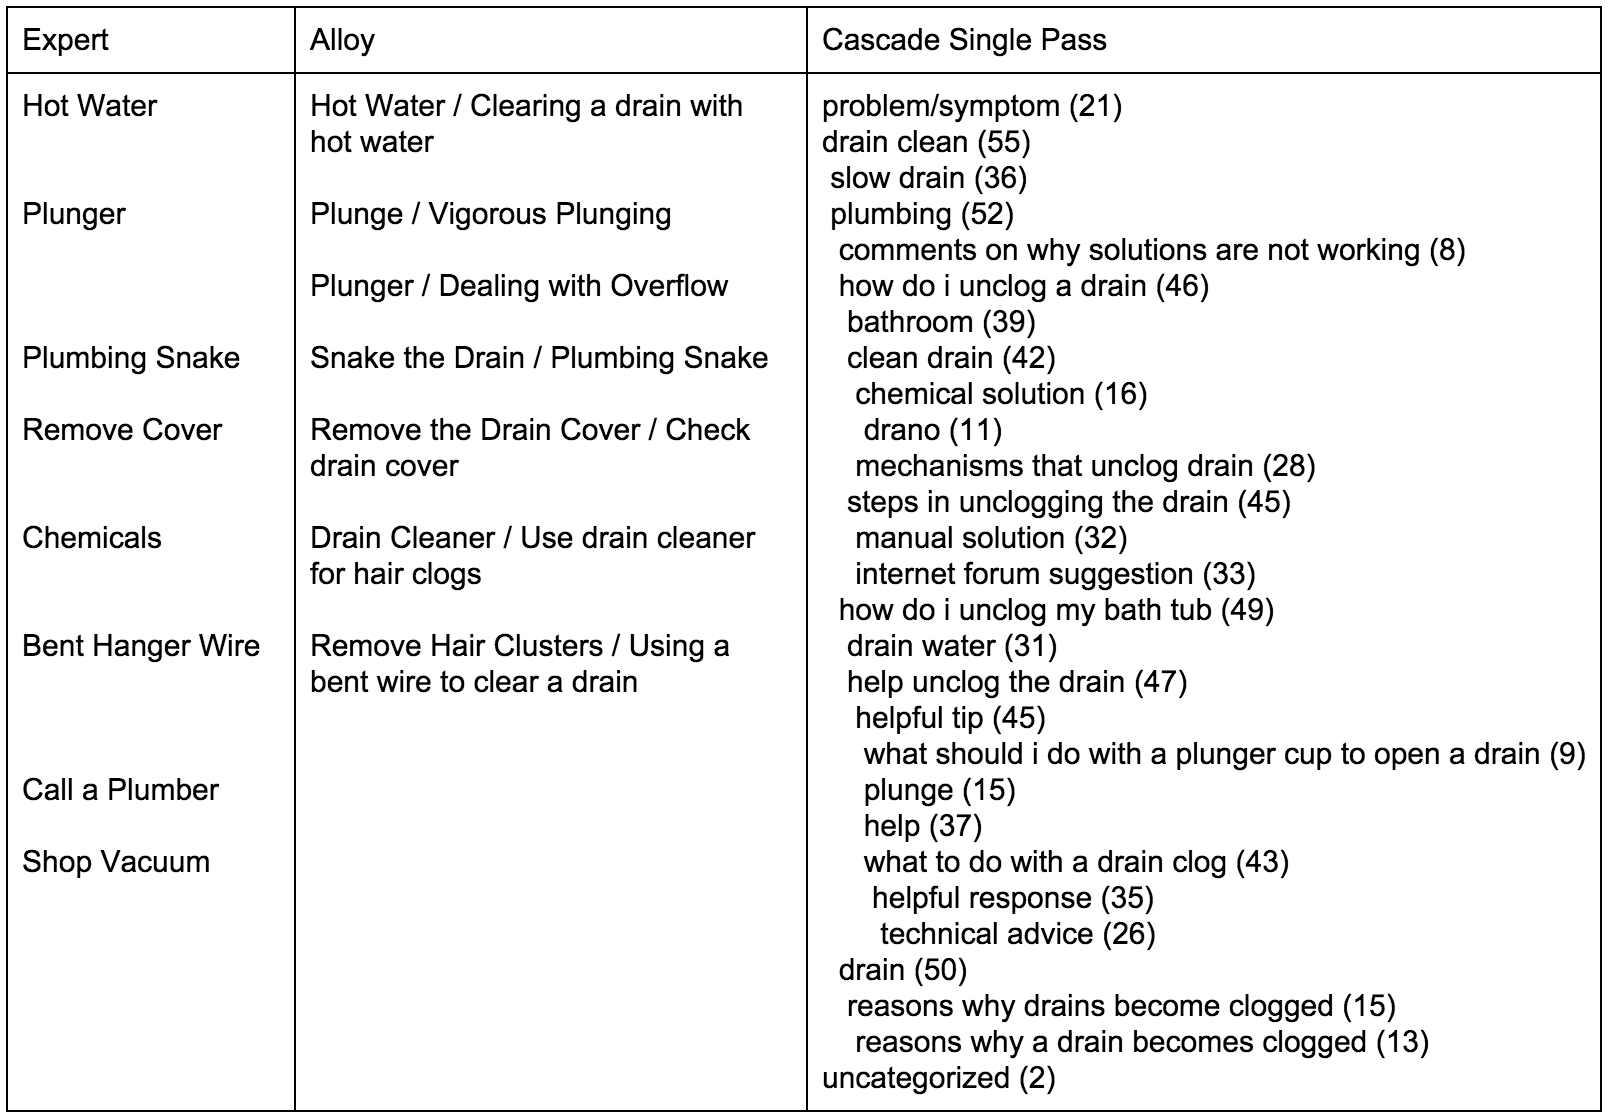
\includegraphics[width=0.9\columnwidth]{Chapters/Alloy/images/bathtub_cats.png}
	\caption{Categories comparison for Q1}
	\label{fig:bathtub_cats}
\end{figure}

%\begin{figure}
%	\centering
%	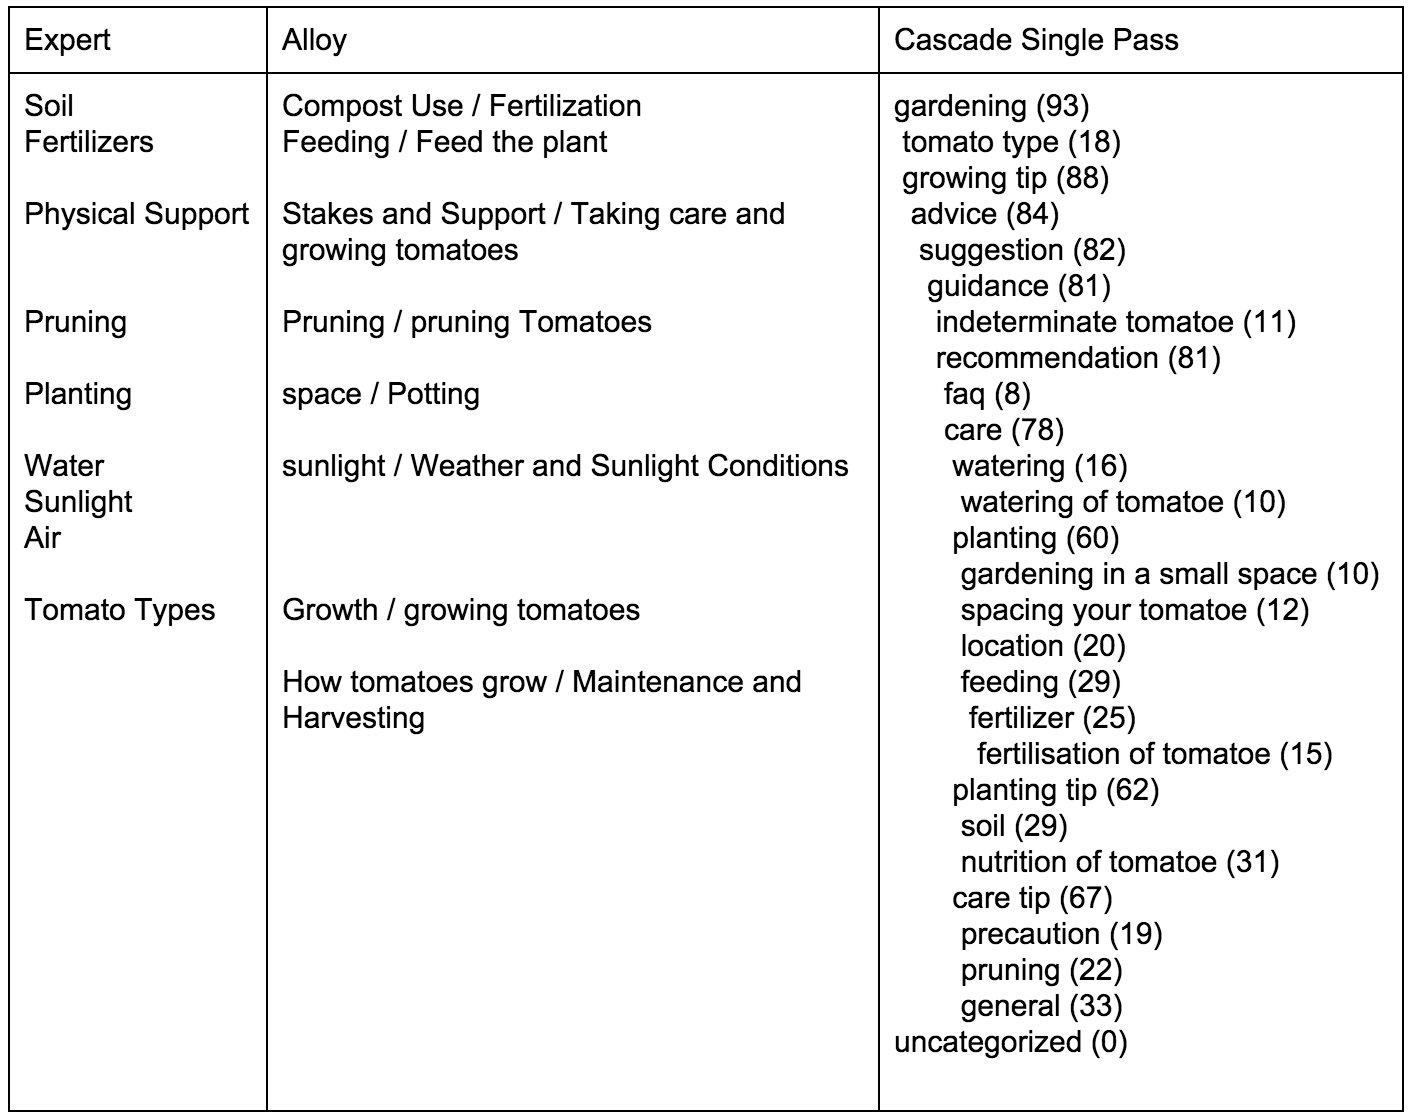
\includegraphics[width=0.9\columnwidth]{images/tomato_cats.png}
%	\caption{Categories comparison for Q2}
%	\label{fig:tomato_cats}
% \end{figure}

We compare Alloy with Cascade using datasets Q1-Q4, a popular crowd-based method for
discovering taxonomies in unstructured data based on overlapping crowd
clusters \cite{chilton2013cascade}.
We implemented a simplified version of Cascade using the parameters
described in the paper, but with only one recursion.  We acknowledge that fine
tuning and multiple recursion might improve Cascade's performance, but the
numbers from our evaluation are consistent with the results reported in the
Cascade paper based on the same metric and similar datasets.

On average, 84\% of categories generated with Alloy were shared with clusters
in the gold standard, versus 50\% for Cascade.  Cascade produced soft
clusters where child clusters did not necessarily have all the items included in
their parents, which breaks the assumptions of using NMI. To produce
a direct comparison, we use the gold standard to greedily extract best
matching, overlapping clusters that cover all items, and evaluated them using
the average F1. In essence, this simulates an omniscient ``oracle'' that gives
Cascade the best possible set of cluster matches, and so is perhaps overly
generous but we wanted to err on the conservative side. The average F1 scores
for each questions using Alloy are .72, .54, .48, .52, and using Cascade are
.50, .48, .42, .39, showing a consistent advantage across questions.
Furthermore, Alloy achieved this better performance at a
lower cost (average \$20 for Alloy vs \$71 for Cascade),
suggesting that machine learning can provide valuable scaling properties.
We show categories created by experts and elicited from the two systems
in Figure~\ref{fig:bathtub_cats} to give a better sense of the datasets and the output.
% and  Figure~\ref{fig:tomato_cats}. 

% \begin{table*}
%   \centering
% 
% \begin{tabular}{ |l|l|p{3in}| }
% \hline
% Expert & Alloy & Cascade Single \\
% \hline
% Hot Water & Hot Water / Clearing a drain with hot water & \\
% Plunger   & Plunge / Vigorous Plunging & \\
%           & Plunger / Dealing with Overflow & \\
% Plumbing Snake & Snake the Drain / Plumbing Snake & \\
% Remove Cover   & Remove the Drain Cover / Check drain cover & \\
% hemicals       & Drain Cleaner / Use drain cleaner for hair clogs & \\
% Bent Hanger Wire & Remove Hair Clusters / Using a bent wire to clear a drain & \\
% Call a Plumber & & \\
% Shop Vacuum & & 
% \multirow{-9}*{
% \begin{minipage}{3in}
% problem/symptom (21)\newline
% drain clean (55)\newline
% \hspace{1mm} slow drain (36)\newline
% \hspace{1mm} plumbing (52)\newline
% \hspace{1mm} \hspace{1mm}  comments on why solutions are not working (8)\newline
%   how do i unclog a drain (46)\newline
%    bathroom (39)\newline
%    clean drain (42)\newline
%     chemical solution (16)\newline
%      drano (11)\newline
%     mechanisms that unclog drain (28)\newline
%    steps in unclogging the drain (45)\newline
%     manual solution (32)\newline
%     internet forum suggestion (33)\newline
%   how do i unclog my bath tub (49)\newline
%    drain water (31)\newline
%    help unclog the drain (47)\newline
%     helpful tip (45)\newline
%      what should i do with a plunger cup to open a drain (9)\newline
%      plunge (15)\newline
%      help (37)\newline
%      what to do with a drain clog (43)\newline
%       helpful response (35)\newline
%        technical advice (26)\newline
%   drain (50)\newline
%    reasons why drains become clogged (15)\newline
%     reasons why a drain becomes clogged (13)\newline
% uncategorized (2)\newline
% \end{minipage}
% } \\[3.1in]
% \hline
% 
% \end{tabular}
%   \caption{Bathtub Categories}
%   \label{tab:bathtub_cats}
% \end{table*}




% \subsection{Crowdworkers}

% The crowdworkers employed to test the proposed method are recruited from Amazon
% Mechanical Turk. With a total of 65 unique workers participated in the
% experiments, 56 of them have IP addresses origin in the United States, 6 of
% them from India, and 3 from other regions. From self-reporting, 40 workers are
% males and 25 workers are females, 8 workers are between the age of 18 to 24, 40
% workers are between the age of 25 to 34, 15 workers are between the age of 35
% to 44, and the rest in other ranges or chose not to report. Each worker is paid
% 1.00 USD for completing one of the two HITs. Therefore, the costs for both
% Workflow2 and Workflow1 is 20.00 USD.

% \begin{table*}
%   \centering
% % question, number of sources, number of clips, number of turkers
%   \begin{tabular}{ c l l l l l }
%     \hline
% 	\tabhead{} &
% 	\tabhead{Phase A Mean} &
% 	\tabhead{Phase A Std. Dev} &
% 	\tabhead{Phase B Mean} &
% 	\tabhead{Phase B Std. Dev} &
% 	\tabhead{ANOVA P-Value} \\
%     \hline

% 	Interface & 4.2270 & 0.6477 & 3.710 & 0.783 & $\sim$ 0.000 \\ 
% 	Instructions & 4.0286 & 0.9592 & 3.786 & 1.001 & $\sim$ 0.156 \\
% 	Difficulty & 3.5099 & 1.0255 & 3.119 & 1.109 & $\sim$ 0.033 \\

%     \hline

%   \end{tabular}
%   \caption{Survey feedback from the crowdworkers.}
%   \label{tab:feedback}
% \end{table*}


% \subsection{Survey feedback from Crowdworkers}
% Upon completion of each HIT, we asked each unique worker to rate the task
% description, interface design, and overall difficulty of the HITs by filling
% out a survey form. We used a 5-point Likert scale, ranging from ``Strongly
% Agree'' (5) to ``Strongly Disagree'' (1) in order to gauge their opinions
% regarding the different features of the HIT. As shown in Table \ref{tab:feedback}, workers
% thought that the interface from Phase A was easier to utilize than interface
% for Phase B (p-value $\sim$ 0.000), with their average response being that they
% agreed that Phase A's interface was easy to use, while Phase B's interface
% was acceptable. There was not a significant difference between their responses
% regarding the instructions, agreeing that for both phases the instructions were
% easy to understand and follow. Finally, workers thought that Phase A was easier
% than Phase B (p-value $\sim$ 0.033), with neither task being considered to be
% particularly easy to complete. 

% We also allowed the Crowdworkers to comment on the HITs, and many of them find
% the clustering process interesting and enjoyable, leaving comments such as
% ``This was an interesting hit. I enjoyed it.'', ``very interesting to name each
% clusters'', and ``This was an interesting study and I actually learned a new
% tip to try and clear a clogged drain.'' 


%\begin{table*}
%  \centering
%% question, number of sources, number of clips, number of turkers
%  \begin{tabular}{ l r r r r r }
%    \hline
%	\tabhead{Questions} &
%	\tabhead{strongly agree} &
%	\tabhead{agree} &
%	\tabhead{neither...} &
%	\tabhead{disagree} &
%	\tabhead{strongly disagree} \\
%    \hline
%    \multicolumn{6}{c}{\tabhead{Phase A}} \\
%    \hline
%	% 54
%	\emph{I find this task easy to complete} & 11\% & 46\% & 31\% & 11\% & 0\% \\
%  
%	% 53
%	\emph{The instructions clearly explain the task} & 34\% & 55\% & 8\% & 4\% & 0\% \\
% 
%	% 54
%	\emph{The user interface is easy to learn and use} & 40\% & 56\% & 4\% & 0\% & 0\% \\
%    \hline
%    \multicolumn{6}{c}{\tabhead{Phase B}} \\
%    \hline
%	% 54
%	\emph{I find this task easy to complete} & 9\% & 45\% & 9\% & 36\% & 0\% \\
%
%	% 53
%	\emph{The instructions clearly explain the task} & 18\% & 55\% & 11\% & 11\% & 11\% \\
%
%	% 54
%	\emph{The user interface is easy to learn and use} & 27\% & 55\% & 11\% & 11\% & 0\% \\
%    \hline
%
%  \end{tabular}
%  \caption{Survey feedback from the crowdworkers.}
%  \label{tab:feedback}
%\end{table*}



\begin{figure*}
	\centering
	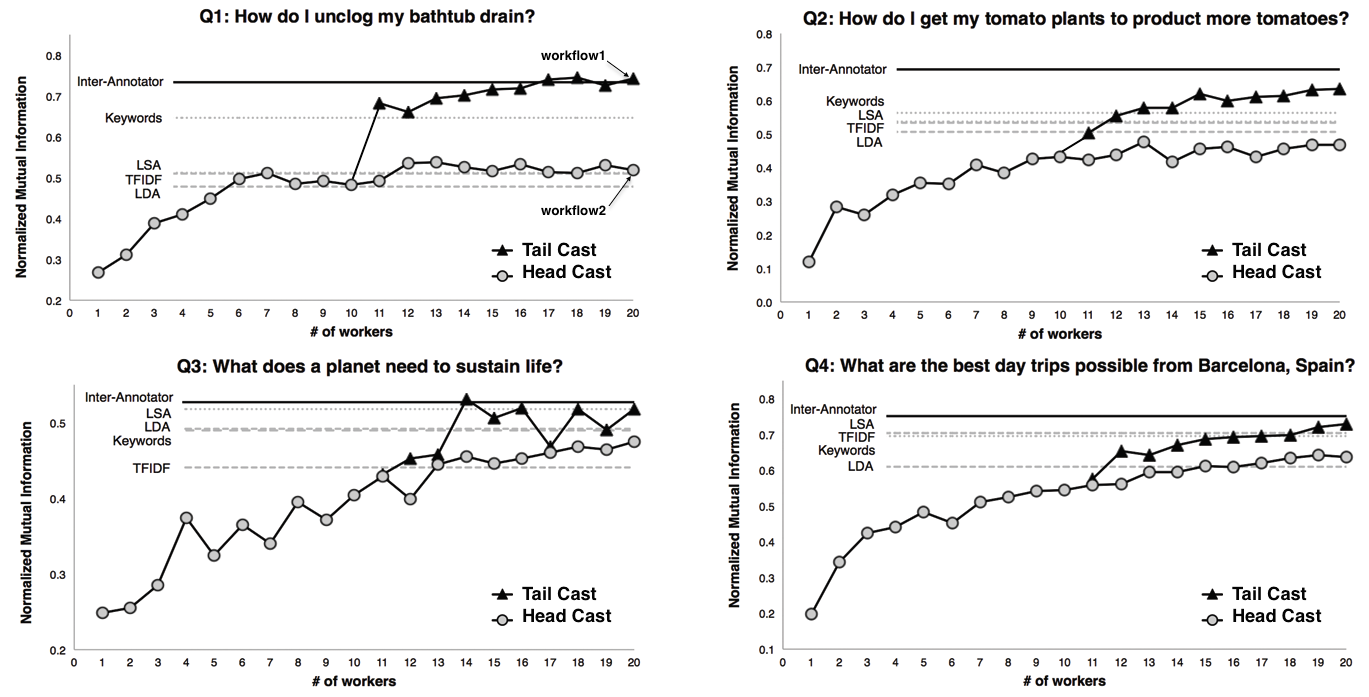
\includegraphics[width=1\columnwidth]{Chapters/Alloy/images/numberOfTurkers.png}
	\caption[Performance comparison of using different number of crowdworkers.]{Performance comparison of using different number of crowdworkers in the Head Cast and the Tail Cast.}
	\label{fig:numberOfTurkers}
\end{figure*}


\subsection{Experiment 2: Robustness}
%!TEX root = main.tex


\footnotetext[1]{We also evaluated Q1 and Q2 using the AMI metric that accounts
    for randomness.  The inter-annotator agreements are .674 and .643,
    respectively, and Alloy performed .674 and .609, respectively. See the
    Evaluation Metric Section for detail.}

% \textbf{Workflow2: $Head Cast$}
% \vspace{-2mm}

In this section, we examine the robustness of
Alloy by varying the number of crowdworkers employed in the Head and the Tail Cast on datasets Q1-Q4. We start
with having only 1 worker in the Head Cast, and evaluate performance as we hire more
workers until we have 20. To test the two phase assumption, in a second
condition, we switch to the Tail Cast after hiring 10 workers in the Head Cast,
and continue to hire 1 to 10 more workers.
This way, we can characterize the cost/benefit trade-offs in hiring different amount of human
judgments. Further, by omitting the Tail Cast completely 
in the first condition, we can verify
the two phase assumption by comparing the performance of a two-phase process
(Head Cast and Tail Cast) with a one-phase control (Head Cast only) while equaling
the number of workers:

\begin{itemize}
    \setlength\itemsep{0.0em}
	\item \emph{Workflow1}. The workflow with ten crowdworkers each for
		the Head Cast and the Tail Cast. Each HIT costs 1 USD.
	\item \emph{Workflow2}. The workflow with twenty crowdworkers and
		the Head Cast only. Each HIT costs 1 USD.
\end{itemize}

In addition, to test how robust Alloy is to the variance of crowdworkers on Amazon Mechanical Turk, 
we also hired eleven sets of ten different crowdworkers (a total of 440) for each 
Head and Tail Casts for Q1 and Q2. 

\subsubsection*{Results}


In Figure~\ref{fig:numberOfTurkers}, we show the performance of
employing different number of workers in the Head and the Tail Cast.  Initially,
increasing the number of workers in the Head Cast shows significant
performance improvements.  However, after gathering training data from around 10 
workers, the performance gain from hiring additional
crowdworkers decreases notably. Instead, performance improved significantly
even with only a few additional crowdworkers in the Tail Cast to refine
the clusters. Overall, 
having
10 crowdworkers in each of the Head and Tail Cast consistently outperformed having all
20 crowdworkers in the Head Cast across all four questions (Table~\ref{tab:results}),
suggesting there is significant value in the Tail Cast.

For Q1 and Q2, we also ran Alloy eleven times using different
crowdworkers, and compared the results against the gold-standard labels and also with
each other. Comparing to the gold-standards, which have inter-annotator
agreements of $.734$ and
$.693$ for Q1 and Q2 respectively, Alloy produced an average NMI of .759 (SD=.016) and .687 (SD=.016), respectively.
Further, the average pair-wise NMI score of the 11 runs are .819 (SD=.040), and .783 (SD=.056), respectively, suggesting Alloy
produces similar results using different crowdworkers on the same datasets.

%Further, the average pair-wise NMI score of the four conditions (Head Cast Q1, Q2, and Tail
%Cast Q1, Q2) are .740 (SD=.106),
%.758 (SD=.088), .819 (SD=.040), and .783 (SD=.056). This suggests Alloy
%produces similar results using different crowdworkers on the same dataset. 



\subsection{Experiment 3: Other Datasets}
%!TEX root = main.tex

% \textbf{Workflow1:} $HeadCast \rightarrow MergeCast \rightarrow TailCast$
% \vspace{-2mm}

%Alloy was initially designed to organize corpora of ideas that answer a specific questions described using short text clips.
In this experiment, we use the same distributed workflow to test Alloy 
using the Wiki and CSCW datasets as described in the Dataset Section, in order
to test how Alloy generalizes to other types of data. These datasets contain long
academic documents or editorial discourses that are infeasible to present multiple items to the crowdworker in one HIT.
Instead, we show a small portion of each item in the datasets to the crowdworkers.
For each item
in the Wiki dataset, we display the thread-starter post and the first two replies. For the CSCW dataset,
we present the abstract
section of each paper, and compare results with the official conference sessions. Machine baselines were however given
access to all of the text of the paper and the full discussion threads in order to provide a strong test of Alloy's approach.

%\niki{move this to discussion if you want}
%We acknowledge that organizing long documents is a limitation of Alloy.
%However, this limitation also presents in most previous crowd-based approaches.

\subsubsection*{Results}

% \subsubsection{CSCW Conference Papers}

For the CSCW dataset, Alloy outperformed all machine baseline
systems with \emph{.748} NMI score using conference sessions as the gold standard Table~\ref{tab:results}.
The Keyword baseline outperformed the TF-IDF baseline (\emph{.652} vs \emph{.584}), showing
that the crowdworkers are extracting valuable keywords in the Head Cast, despite that
research papers may be difficult or impossible for crowdworkers to understand. On the other hand,
Alloy produced 24 categories out of 135 abstracts, more than all other datasets. One possible
assumption is that it may be more difficult for novice workers to induce abstract categories
when organizing expert dataset, leading to higher number of more lower level categories in
the outcome.

% Note that even though only the abstract sections were available to the crowdworkers,
% we used the full articles as the input to the baseline systems to improve their performance,
% and explored multiple parameter settings report their best results.

% \subsubsection{Wikipedia Editor Discussion Threads}

For the Wiki dataset, the NMI score between annotators was \emph{.604}, which is comparable
to the two other large datasets Q5 and Q6. Comparing to the two sets of expert
labels independently, Alloy's output measured \emph{.528} and \emph{.507}.
Compared to all previous results, Alloy seemed to perform less favorably on this
dataset. As mentioned in the Dataset Section, the raters found the this dataset the most
difficult to organize, as there are many different valid structures that the two
annotators were unable to reach an agreement 
also hints that the space of valid solutions may be larger on this dataset. 
In addition, we only showed the first three comments of
each discussion to the crowdworkers, whereas the annotators and the machine baselines
have access to the full discussion. 
We acknowledge length of items is a limitation, and will discuss in detail in
the Discussion Section.

%This is potentially a substantial disadvantage to
%Alloy, as the full discussions can contain up to more than a hundred comments.
%Unlike the abstracts of research papers, the first three comments might not be
%representative enough of the discussions.




\section{Application: \textbf{Knowledge Accelerator}}
\label{chap:ka}

{\rmfamily
This work was previously published in ACM SIGCHI 2016 \cite{ka} and has been adapted for this document.
}

\begin{figure}
    \centering
    \frame{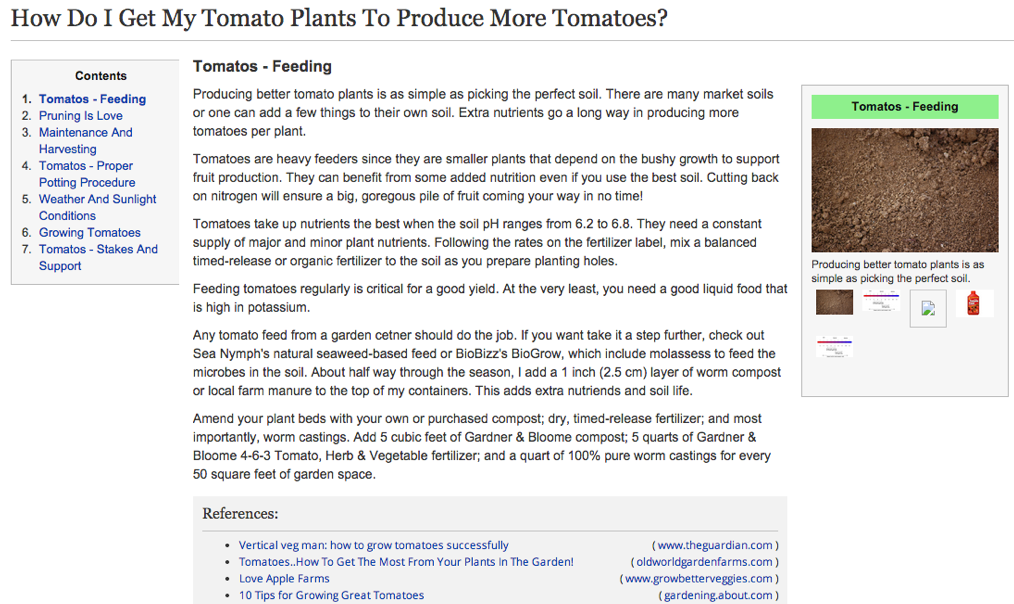
\includegraphics[width=1\columnwidth]{Chapters/KA/final_answer}}
    \caption[Alloy clusters synthesized into a report articles using the Knowledge Accelerator.]{Example report synthesized by the Knowledge Accelerator system. The table of content on the left listed cluster names generated from Alloy, each corresponded to a different section in the report.}
    \label{fig:final_answer}
\end{figure}

\begin{figure}
    \centering
    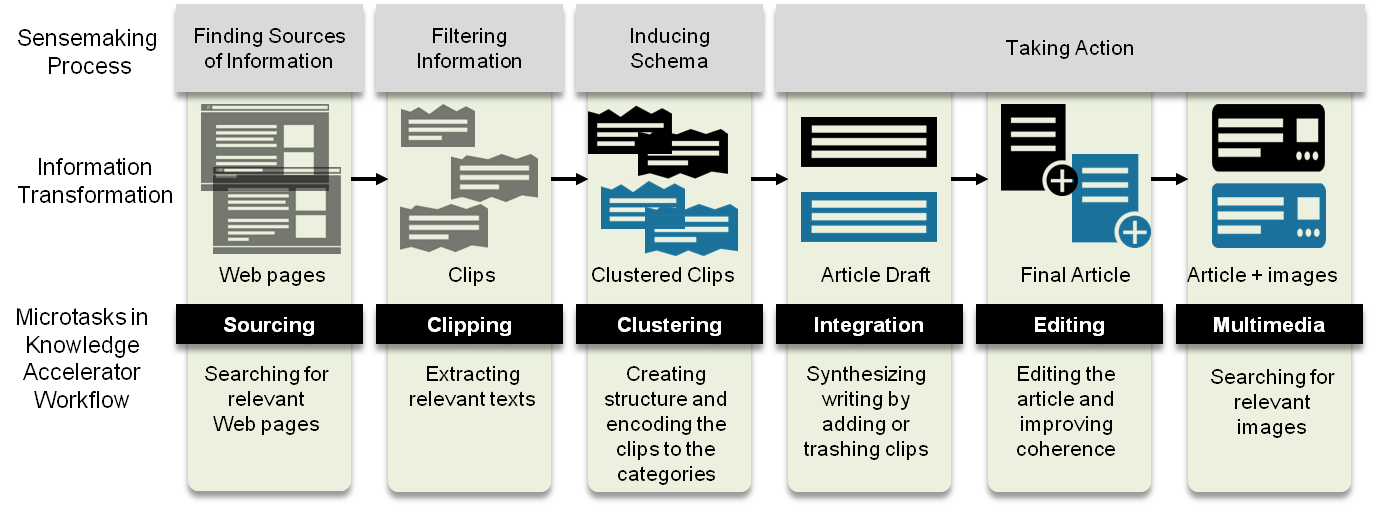
\includegraphics[width=1\columnwidth]{Chapters/KA/overview}
    \caption[The Knowledge Accelerator (KA) with Alloy as the Clustering Stage.]{The process of the Knowledge Accelerator (KA). Alloy is used for the Clustering Stage of the pipeline.}
    \label{fig:process}
\end{figure}


To evaluate the usefulness of structures generated by Alloy in a more realistic scenarios, we first used Alloy to clusters a larger set of information seeking datasets (Table~\ref{tab:evaluation}) collected using the same procedure as described in \cref{chap:info_seek_datasets}. We then developed a prototype system called the ``Knowledge Accelerator'' (KA) to synthesize the output of Alloy into articles. Each of the cluster produced by Alloy corresponds to a different section in an article. An example of the output of the system for the target question ``How do I get my tomato plants to produce more tomatoes?'' can be found in Figure~\ref{fig:final_answer}.

In addition, the KA system probes how to accomplish a complex information synthesis task entirely through relatively small contributions. We limited our maximum task payment to \$1 US, aimed at incentivizing a Target task time of approximately 5-10 minutes. Critically, the KA system accomplishes this process without a core overseer or moderator. Figure \ref{fig:process} shows the overview of the KA System with Alloy being the Clustering Stage. For more details on the KA system refer to \cite{ka}.

We evaluated the usefulness and coherence of the articles by comparing them against webpages an individual might use if they were to complete the same tasks without KA and Alloy --- Top Google search results that consists of expert-written articles published by trusted sources such as CDC.gov or the New York Times, as well as popular online forums such as TripAdvisor and Yahoo Answers.

\subsection{Experimental Settings}

Eleven topics were selected for evaluation by browsing question and answer forums, Reddit.com, and referencing online browsing habits \cite{pewReport}. For questions Q3 and Q8 we added additional constraints (i.e., having kids and age) to test the performance of the system for more personalized questions.
To compare the two conditions, participants were recruited through the Amazon Mechanical Turk US-only pool and paid \$1.50 for rating two webpages. Each participant was randomly assigned an output article from KA and a top search result webpage for the same topic (Figure~\ref{fig:aggregated}), and rate both webpages based on six criteria using 7-point Likert scale questions and provided free-form explanations: \emph{comprehensiveness}, \emph{confidence}, \emph{helpfulness}, \emph{trustworthiness}, \emph{understandability}, and \emph{writing}. We averaged ratings on these dimensions into a single score representing the overall perceived quality of the page.


\begin{table}
  \centering
  \footnotesize
% question, number of sources, number of clips, number of turkers
  \begin{tabular}{l r l}

	Question &
	\multicolumn{1}{c}{N} &
    \multicolumn{1}{c}{Score} \\
    \hline
	% 102
	\multicolumn{1}{p{0.75\columnwidth}}{\textbf{Q1}: \textit{How do I unclog my bathtub drain?}}
	& 116 & ~0.292 * \\

	% 115	
	\multicolumn{1}{p{0.75\columnwidth}}{\textbf{Q2}: \textit{How do I get my tomato plants to produce more tomatoes?}}
	& 177 & ~0.420 * \\

	% 153
	\multicolumn{1}{p{0.75\columnwidth}}{\textbf{Q3}: \textit{What are the best attractions in LA if I have two little kids?}}
	& 158 & -0.044 \\

	% 116
	\multicolumn{1}{p{0.75\columnwidth}}{\textbf{Q4}: \textit{What are the best day trips possible from Barcelona, Spain?}}
	& 98 & -0.109 \\

	% 177
	\multicolumn{1}{p{0.75\columnwidth}}{\textbf{Q5}: \textit{My Worcester CDi Boiler pressure is low. How can I fix it?}}
	& 139 & ~0.878 * \\

	% 168
	\multicolumn{1}{p{0.75\columnwidth}}{\textbf{Q6}: \textit{2003 Dodge Durango has an OBD-II error code of P440. How do I fix it?}}
	& 138 & ~0.662 * \\

	% 175
	\multicolumn{1}{p{0.75\columnwidth}}{\textbf{Q7}: \textit{2005 Chevy Silverado has an OBD-II error code of C0327. How do I fix it?}}
	& 135 & ~0.412 * \\

    % 160
	\multicolumn{1}{p{0.75\columnwidth}}{\textbf{Q8}: \textit{How do I deal with the arthritis in my knee as a 28 year old?}}
	& 139 & ~0.391 * \\

    % 161
	\multicolumn{1}{p{0.75\columnwidth}}{\textbf{Q9}: \textit{My Playstation 3 has a solid yellow light, how do I fix it?}}
	& 119 & ~0.380 * \\

    % 162
	\multicolumn{1}{p{0.75\columnwidth}}{\textbf{Q10}: \textit{What are the key arguments for and against Global Warming?}}
	& 138 & ~0.386 * \\

    % 163
	\multicolumn{1}{p{0.75\columnwidth}}{\textbf{Q11}: \textit{How do I use the VIM text editor?}}
	& 138 & ~0.180 \\
    \hline
    \multicolumn{3}{l}{\textbf{*} = significant at $p < 0.01$ after Bonferroni correction}\\

  \end{tabular}
  \caption[Comparing KA output with top websites for the eleven questions.]{Average difference between the KA output and top websites for the eleven questions (positive indicates higher ratings for KA, negative indicates higher ratings for the competing website). Each rating was an aggregate of 6 questions on a 7-point Likert scale.}
  \label{tab:evaluation}
\end{table}

\begin{figure}
    \centering
    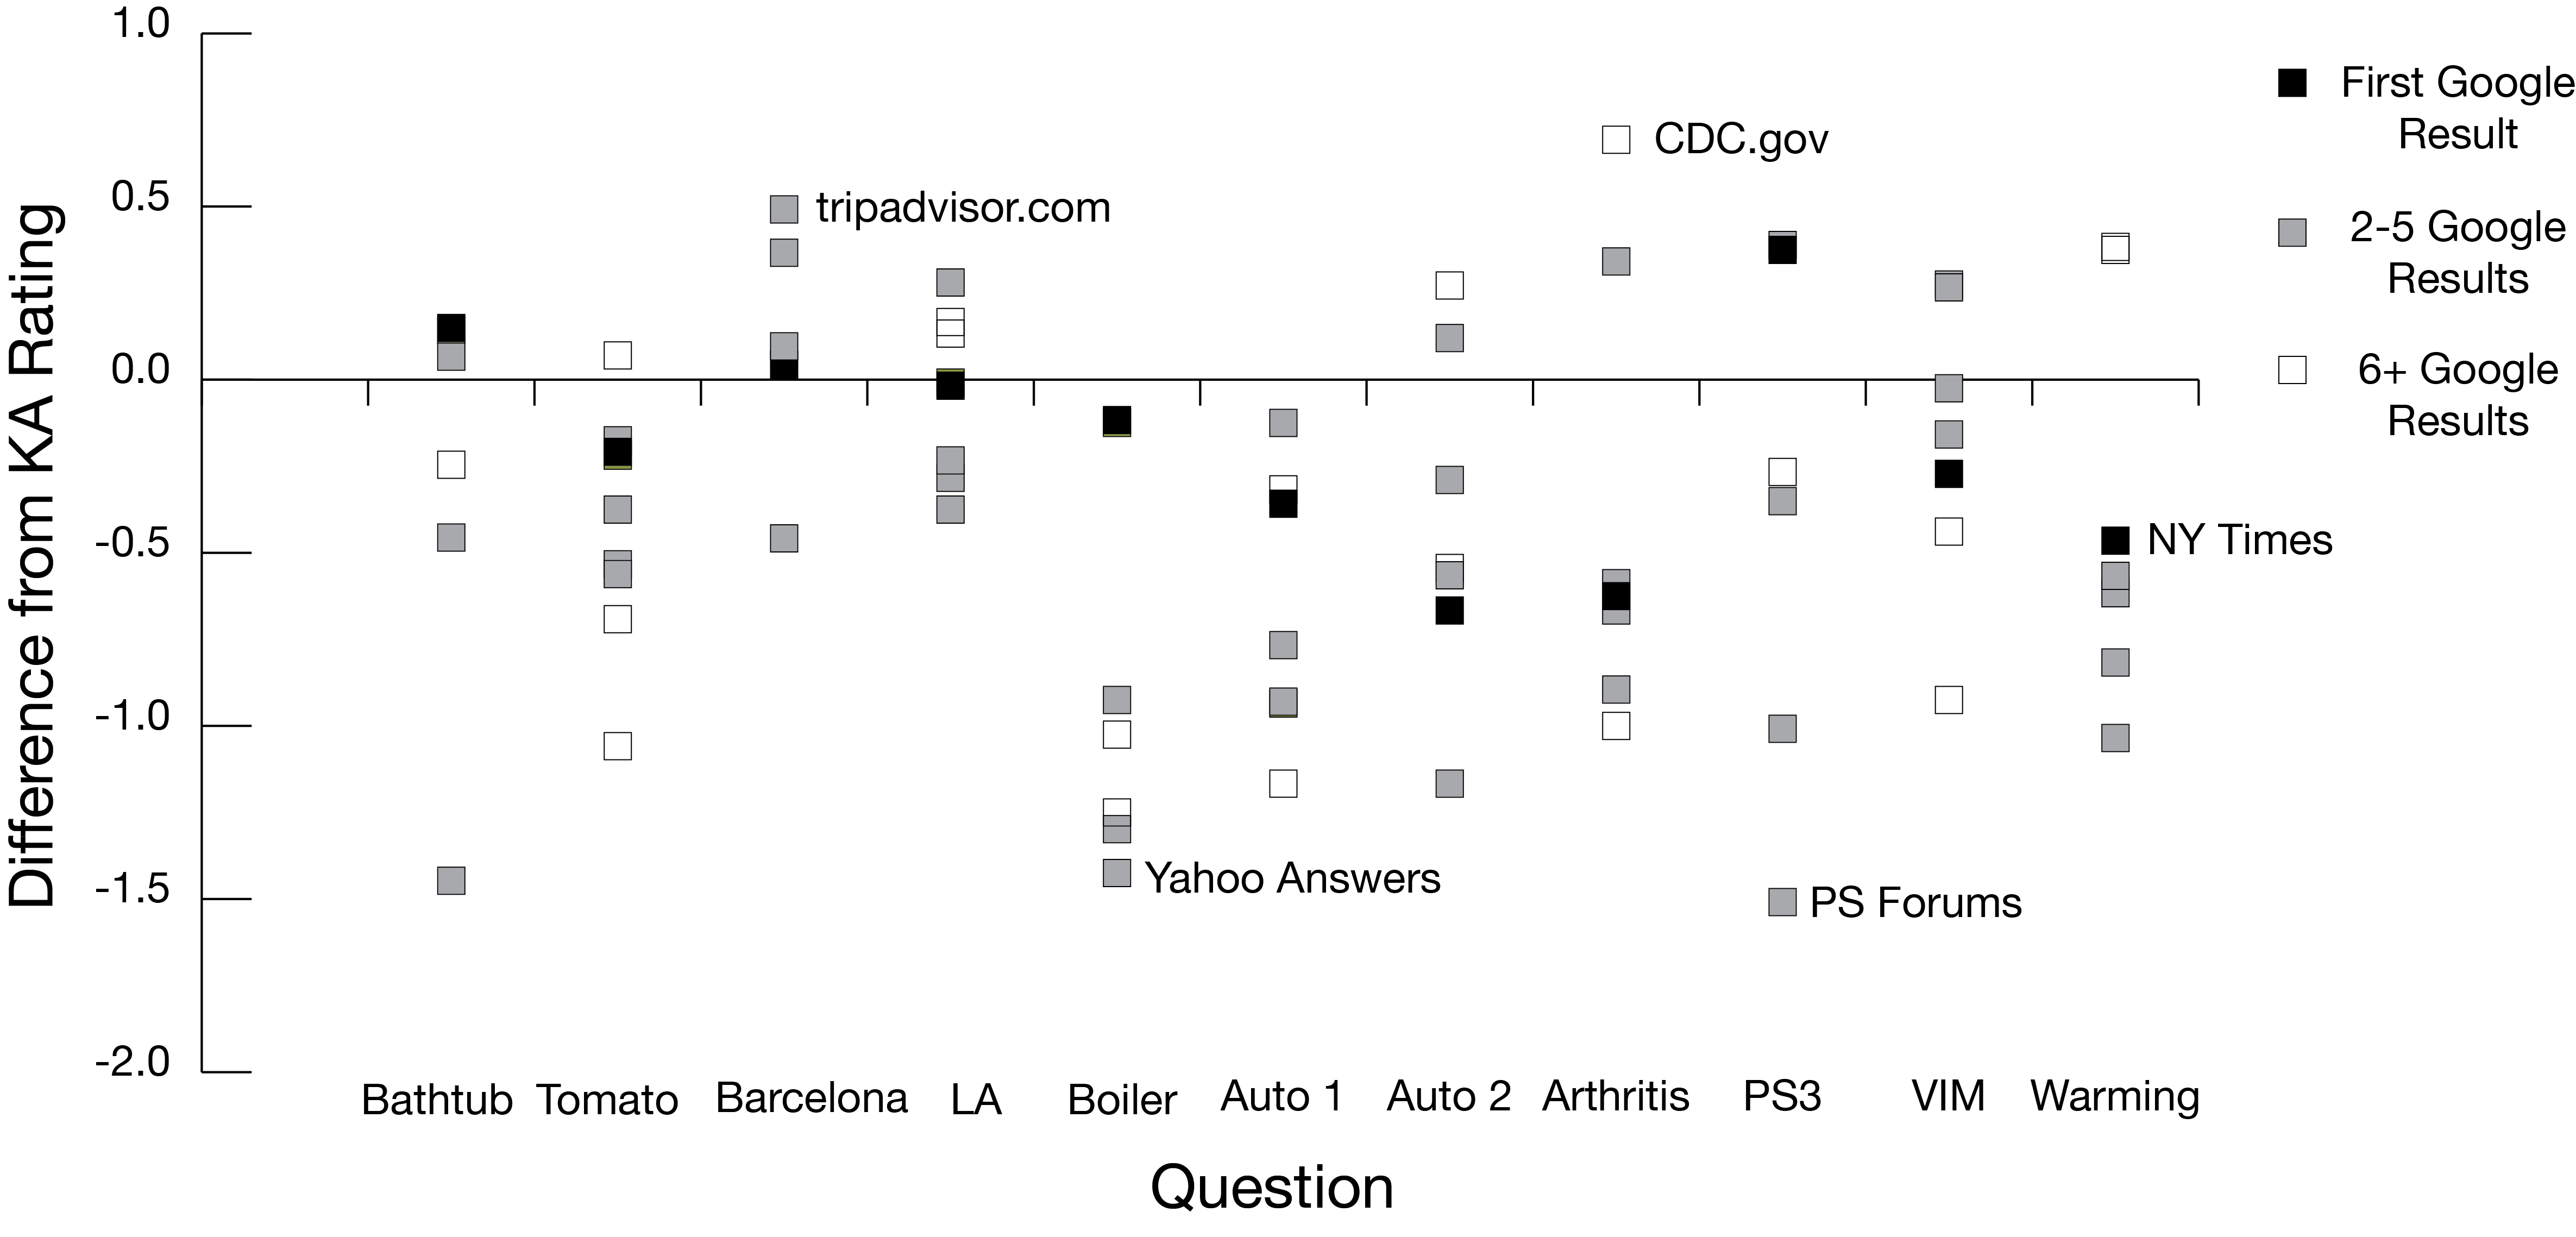
\includegraphics[width=1\columnwidth]{Chapters/KA/source_eval_graph}
    \caption[Results across questions and websites.]{Results across questions and websites. Points represent the average aggregate score difference between the KA answer and an existing site}
    \label{fig:aggregated}
\end{figure}

\subsection{Results}

\begin{table}
  \centering
  \small
% question, number of sources, number of clips, number of turkers
  \begin{tabular}{lrrr}
    \hline
    \textbf{Phase} & \textbf{Task Pay} & \textbf{Avg. \# of Tasks} & \textbf{Avg. Cost} \\
    \hline
	Sourcing & \$0.25 & 15 & \$3.75 \\

    Clipping & \$0.50 & 21.6 & \$10.80 \\

    Alloy Head Cast & \$1.00 & 10 & \$10.00 \\

    Alloy Merge + Tail Cast & \$1.00 & 10 & \$10.00 \\

    Integrate & \$0.50 & 37.2 & \$18.60 \\

    Edit 1 & \$0.75 & 28.8 & \$21.60 \\

    Edit 2 & \$1.00 & 28.8 & \$28.80 \\

    Images & \$0.50 & 9 & \$4.50 \\
    \hline    
    \textbf{Total} & & 160.4 & \$108.05 \\
    \hline
  \end{tabular}
  \caption[Average number of worker tasks and cost of running KA.]{Average number of worker tasks and average cost per phase, and overall, to run a question.}
  \label{tab:cost}
\end{table}

The costs of running a question through the KA system is shown in Table~\ref{tab:cost}. Across the 11 topics we tested, a full run with around 100 short text clips costed an average of \$108.50, of which around \$15 is spent on searching and extracting the text clips from webpages, \$20.00 is spent by the Alloy system, and the rest on synthesizing each of the Alloy clusters into a section in the final article and making sure the different sections are coherent.

Aggregating across all questions, KA output was rated significantly higher than the top 5 Google results (KA: $\bar{x} = 2.904$ vs Alt. Sites: $\bar{x} = 2.545$, $t(1493) = 13.062$, $p < 0.001$). An analysis of individual questions corrected for multiple comparisons is shown in Table~\ref{tab:evaluation}. 

The strongly positive results found were surprising because some of the websites in the comparison set were written by experts and had well-established reputations. Only on the two travel questions, Barcelona ($\bar{x} = -0.109$) and LA ($\bar{x} = -0.044$), and the VIM question ($\bar{x} = 0.180$) did the KA output not significantly outperform the comparison pages. A closer examination of these pages suggests that for the two travel questions, because of the strong internet commodity market surrounding travel, a considerable amount of effort has been spent on curating good travel resources. Even with the slightly more specific LA query, there were still two specialized sites dedicated to attraction for kids in LA (Mommypoppins.com and ScaryMommy.com). The VIM question represented a mismatch between our output and the question style. A number of the sources for the question were tutorials, however in the clipping phase, these ordered tutorials were broken up into unordered clips, creating an information model breakdown. This points out an interesting limitation in the KA approach, and suggests that adding support for more structured answers (e.g., including sequential steps) could be valuable future work. 


%As an additional external evaluation, for the two questions (Q6 and Q7) related to automotive systems we compared the discovered categories from the KA system with two commercial knowledge service products generated by expert technicians. We compared the KA response's accuracy and comprehensiveness, and found that it discovered all the categories referred to in these two commercial products for each question. Furthermore, the categories from the KA output provided more categories not mentioned in the commercial product (average 2.5 categories from two commercial products, while average 9.5 categories from KA). We validated these additional categories with expert automotive professionals who evaluated them as also being plausible and reasonable for the given questions. There was one instance in which two distinct categories (Encoder Motor and Encoder Motor Sensor) from the commercial products were clustered into the single category named Encoder Motor Assembly in the KA output. However, the full text answer from the KA system for Encoder Motor Assembly did still contain these two sub-components with different repair procedures. 

%It may seem surprising that KA would work well for questions such as automotive error codes, where the response relies heavily on technical knowledge and jargon. On further inspection we believe this is because there are many online resources that have valuable information pertaining to these questions but are in unstructured and dialog oriented forms. Workers in the sourcing phase found rich sources of online information from many car enthusiast discussion forums, in which members tried to diagnose and help each other solve their automative problems. Although crowd workers may not understand the esoteric jargon of the automative domain, their understanding of grammar, semantics, and argument structure was sufficient to let them find, filter, cluster, integrate, and edit this domain-specific information. These results suggest a interesting avenue for future research leveraging human understanding of semantics and argument structure to extend crowdsourcing to process expert domain knowledge and to understand the limits of where such an approach breaks down.

%(see Figure~\ref{fig:feedback})



%\subsection{Discussion}

 \begin{figure}
 	\fbox{ \vbox{
 		\ttfamily
 		\footnotesize
 		
		\textbf{categories induced during clipping (without Alloy):}\\
 		Boil Water, use hot water, Plunger, try a snake, How to Remove drain stopper, bleach, Use Drano Max Gel, baking soda, drain, tips to unclog, problem, tools, research, internet research, ..., etc.
 		
 		\rule{\columnwidth}{0.1pt}
 		
 		\textbf{categories induced by Alloy:}\\
 		Hot Water, Plunge, Plunger, Snake the Drain, Remove the Drain Cover, Drain Cleaner, Remove Hair Clusters.
 		
 		\rule{\columnwidth}{0.1pt}
 		
 		\textbf{gold-standard categories:}\\
 		Hot Water, Plunger, Plumbing Snake, Remove Cover, Chemicals, Bent Wire Hanger, Call a Plumber, Shop Vacuum.
 	}}
 	\caption[Categories induced from different stages of KA.]{Categories induced from different stages for Q1: \textit{How do I unclog my bathtub drain?}}
 	\label{fig:delayed-structuring}
 \end{figure}

The strong performance of the system is perhaps surprising given that its output was generated by many non-expert crowd workers, none of whom saw the big picture of the whole, and Alloy is a core component that provided useful and coherent structures for producing the final report. Initially we had workers provide labels to categorize each clip, which we planned to use to develop a structure for the article. However, the lack of context of the bigger picture made these labels poorly suited for inducing a good structure. For example, in Figure~\ref{fig:delayed-structuring} the top box shows the category structure induced by crowdworkers during clipping and without using Alloy during clipping, categories induced using Alloy, and gold standard categories developed by two independent annotators with access to all clips and sources, respectively. Categories induced without using Alloy matched poorly with the gold standard categories, and include categories with very different abstraction levels (e.g., \textit{Use Drano Max Gel} vs \textit{tips}). On the other hand, Alloy produced categories that were more coherent and matched more with gold-standard categories.

While we do not believe that this should be interpreted as a replacement for expert creation and curation of content, instead, the power of the system may actually be attributable to the value created by those experts by generating content which the crowd workers could synthesize and structure into a coherent digest. This explanation suggests that the approach would be most valuable where experts generate a lot of valuable information that is unstructured and redundant, such as the automative questions in which advice from car enthusiasts was spread across many unstructured discussion forums. In contrast, KA's output did not outperform top web sources for topics such as travel, where there are heavy incentives for experts to generate well structured content.  We believe its performance is likely due to its aggregation of multiple expert viewpoints rather than particularly excellent writing or structure per se, never the less, the KA system showcased that the structures produced by Alloy can be synthesized into coherent articles that were useful for exploratory searchers.



\section{Discussion}
%!TEX root = main.tex


In this chapter, we took a step towards tackling
the problem of clustering high-dimensional, 
short text collections by combining techniques from natural language processing and
crowdsourcing.  By using a two-phase process connected by a machine learning backbone,
our proposed method compensates
for the shortcomings of crowdsourcing (e.g., lack of context, noise) and
machine learning (e.g., sparse data, lack of semantic understanding). As part of the system we introduced an approach aimed at providing greater context to workers by transforming their task from clustering fixed subsets of data to actively sampling and querying the entire dataset. 

We presented three evaluations that suggest Alloy performed better 
and more consistently than automatic
algorithms and a previous crowd method in accuracy with 28\% of the cost
(Exp.1), is robust to poor work with only 20 workers (Exp.2),
and is general enough to support different types of input (Exp.3).
Qualitatively, we noticed Alloy often produced better names for categories than
machine algorithms would be capable of, including names not in the text (e.g., a cluster 
including items about \emph{smart thermostats} and \emph{solar panels} was
named ``\emph{Home Improvements}'' which was not in the actual text).

% On average, Alloy produced results
% with .623 against the gold-standards, .023 lower than the inter-annotator
% agreement,
%which is higher than all four baseline systems that ranged from
% .503 to .554 (Table~\ref{tab:results}).

%The first experiment shows that based on
%manually created gold-standard data outperformed four automatic /
%semi-automatic baseline systems, and produced clusters with normalized mutual
%information scores comparable to human inter-annotator agreement.  
%Alloy also performed better comparing to state-of-the-art crowd-based method 
%on accuracy using 28\% of the cost.
%Compared to some previous crowd-based methods, which rely on earlier
%crowdworkers to conceptualize or generate categories for each items based on
%limited context, our method based on crowdworkers ``voting'' on whether each
%item pair should be in the same cluster is less prone to a few workers making
%bad judgements or creating general but not informative clusters (e.g.,
%\emph{answers} or \emph{tips}). Previous methods also suffer from scaling
%problems as they require each item to be labeled by at least one crowdworker.
%In Phase A of the proposed method, we employ crowdworkers to select salient
%keywords from a small set of clips as general features that can be
%used to cluster clips that are not seen by any crowd worker.
%
%In the second experiment, we test the robustness and the strength of the
%two-phase approach of the proposed method by using different number of
%crowdworkers at different phases. Results show even with only a few workers in
%the second phase can significantly improve the performance. In the third
%experiment, we showed that the distributed version of Alloy can produce
%similar performance on significantly larger datasets.  
%
%In the final experiment, we showed that Alloy can support datasets beyound
%information seeking, by evaluating against datasets extracted from Wikipedia
%and a research conference. Results show that the proposed method is able to
%organize expert documents evaluated based on conference sessions, but not as
%good on Wikipedia editor discussions.


% (limitations)
% we may want to discuss limitations such as how would we scale to very large
% bodies of text or larger documents than snippets, also supporting multiple
% classification and hierarchy.

%\subsection{Limitations and Future Work}

One potential concern might be whether Alloy's tasks take too long to be considered microtasks. 
While Alloy deploys HITs that take more than a few
seconds to finish, we think they are still comparable to other complex microtask systems
such as Soylent \cite{bernstein2010soylent} and CrowdForge \cite{kittur2011crowdforge}.
Specifically, based on a total of 281 HITs, the median run-time
for the Head Cast HITs is 7.5 minutes (M=8,3, SD=4.1), for
Merge Cast 8.3 minutes (M=16.2, SD=15.6), and for Tail Cast
11.4 minutes (M=13.2, SD=6.1). 
Despite having less workers
doing longer tasks, Alloy performed consistently
across different sets of workers on the same datasets.


During development, some assumptions, both explicitly
and implicitly, were made about the input of the system:
1) there are more clips than categories.
2) the categories follow a long-tailed distribution.
3) clips belong to primarily one cluster.
4) there is a small set of gold-standard clusters.
5) workers can understand the content enough to cluster it.
Note that we do not assume the crowdworkers can understand the semantics of the
content, but just enough to identify ideas that are salient and common in the
dataset.
Thus they may be able to cluster complex topics such as machine learning without
understanding those topics if enough relational context is embedded in the clips.
For example, an abstract of a research paper may say ``this paper uses POMDP
machine learning
approaches to cluster text'', they might put it in a ``clustering''
cluster without
knowing what a POMDP is.

% \begin{enumerate}
%     \setlength\itemsep{0.1em}
% 
%     \item there are many more clips than categories.
%     \item the categories follow a long-tailed distribution.
%     \item clips belong to primarily one cluster.
%     \item there is a small set of gold-standard clusters.
%     \item workers can understand the content enough to cluster it.
% \end{enumerate}

One obvious limitation to our approach is clustering long documents.
This is a common limitation for crowd-based systems that rely
on workers reviewing multiple items for context
(either from random selection or active sampling). It becomes infeasible to fit multiple
items in a single HIT if the length of each item is long.
Another related limitation is organizing documents that describe multiple topics. 
Lab studies in a past work \cite{kittur2013costs}
showed that individuals are able to decompose long
documents into short clips of single topics during information seeking tasks. 
One way to expand the
proposed method to overcome the length limitation could be splitting documents into short
snippets, either with the crowds or machine algorithms,
and create topical clusters using Alloy.

% We can more formally characterize the scaling function on the number of categories shown in the Merge
% Cast as $T = log_c~N$, where $c$ represents the sparseness parameter of a dataset, $N$ the number of items 
% in the dataset, and $T$ the number of categories shown in the Merge Cast. The upper-bound limitation of 
% Alloy is then $T < L$, where $L$ is a limit on the complexity of a task given the characteristics of the 
% human computation platform utilized. Intuitively, this means that the Merge Cast will scale better 
% when the dataset involves fewer categories that explain more of the data, and when the human computation 
% platform supports more complex tasks.

% If we formulate the sparseness parameter $c$
% of a dataset base on the number of items $N$
% and the number of categories $T$ as $T = log_c ~ N$, the limitation of the distributed Merge Cast is 
% then $\ell \ge T$, where $\ell$ is the cognition limit of number
% of categories that can be presented in a single post to the given crowdsourcing marketplace.

Another limitation is organizing datasets that are inherently difficult to structure categorically. For example, 
concepts in Q3 (\emph{planetary habitability}) have causal relationships without
clear categorical boundaries (e.g., \emph{distance to sun}, \emph{temperature} and \emph{liquid water}).
As a result, all approaches had significant trouble,
including low agreement between human annotators. 
On the other hand, some dataset can be organized categorically in multiple ways.
In Q4 (\emph{Barcelona}) we found that some categories fit a \emph{place}
schema (e.g., \emph{Sitges}, \emph{Girona}) while other categories fit a \emph{type}
schema (e.g., \emph{museums}, \emph{beaches}).
One approach for addressing this could be trying to cluster workers to separate the different kinds of schemas; however, upon inspection we found that individual
workers often gave mixtures of schemas. This interesting finding prompts further research to investigate what cognitive and design features may be causing this, and how to learn multiple schemas. 
%One possible explanation is that a single schema often only covers part of the dataset,
%and we require the workers to organize all given items. For example, the $tool$ schema
%covers majority of the items in Q1 (bathtub drain), but does not cover items that
%explains how
%drains works, safety precautions, or steps to remove drain covers. 
%Another assumption is that information on the original sources are organize in different %ways, 
%and may influence the workers to use multiple schemes. 
%One possible improvement is to explicitly assign schemes to different workers, 
%and allow them to only cluster items that fits the given scheme. 
%A more interesting direction may be discovering a set of good schema using the crowd. 


% By examining the data, we found two reasons.  First,
% there is a lot of uncertainty in the topic, because not even the science
% community has a clear idea of the answer; for example, some clips even discussed whether
% the definition of life should be exclusively carbon based. Second, there are a
% lot of interconnected and correlated factors. For example, the \emph{distance
% 	to its star} determines whether a planet is in the \emph{habitable zone} of
% a solar system, which effects the \emph{temperature} of the planet and whether
% it potentially contains \emph{liquid water}. 


Looking forward, we identified a set of patterns that may be useful to system designers
aiming to merge human and machine computation to solve problems that involve rich
and complex sensemaking.
%  Our two-phase clustering approach breaks up human involvement
%  such that early workers can focus on building up context and finding common and
%  salient patterns in the data which are useful for training machine learning
%  classifiers, while later stage workers can leverage this previously
%  generated context (in the form of already created categories) to focus on the
%  edge cases and one-offs.
The hierarchical clustering backbone we use to integrate judgments from a
variety of crowdworker tasks allows us to \textit{cast} for different types of
crowd judgments and \textit{gather} them into a coherent structure that
iteratively gets better with more judgments.  We also introduce useful new
patterns for improving global context through self-selected \emph{sampling} and
keyword \emph{searching}.  One important consideration these patterns bring up
is that while previous ML-based approaches to crowd clustering have focused on
minimizing the number of judgments, we have found it is at least as important
to support the rich context necessary for doing the task well and setting up
conditions that are conducive for crowdworkers to induce meaningful structure
from the data.


We hope the patterns described in this chapter can help researchers
develop systems that make better use of human computation in different domains and for different purposes. For example,
the \emph{sample and search} pattern could potentially be adapted to support other tasks such as image
clustering, where crowdworkers could use the sampling mechanism to
get a sense of the variety of images in the dataset, highlight discriminative objects, and label images queried based on features extracted from the highlighted regions. Furthermore, the \emph{cast and gather} 
pattern may provide a useful framework for combining
crowds and computation that is both descriptive and generative. For example, Zensors \cite{laput2015zensors}, a crowd-based real-time video event detector, could be considered a form of the cast and gather pattern which uses a classification algorithm instead of a clustering algorithm as a backbone, and casts for human judgements whenever its accuracy falls below a threshold (e.g., if an environmental change lowers precision), with the classifier backbone retrained with the new human labels. While we used a clustering backbone in this work, 
future system designers might consider other machine learning backbones (e.g., classification or regression algorithms) for different tasks. Overall, we believe this approach takes a step towards solving complex cognitive tasks by enabling better global context for crowd workers and providing a flexible but structured framework for combining crowds and computation.


% Many other future research directions present themselves. For example, we can
% improve quality by using the crowd to fuse similar dimensions together by highlighting
% synonymous words to improve quality. On the other hand, we can push the boundary of crowd-clustering methods by testing Alloy on typical machine learning datasets that have significantly more items. 
% Other computational techniques could be used to optimize Alloy to require
% less human labor. For example, techniques in \cite{bragg2013crowdsourcing}
% can potentially be adapted to dynamically determine when to stop hiring more
% crowdworkers in each Cast. Alternatively, 
% the random sampling mechanism in the Head Cast could be replaced by
% active learning techniques; for example, presenting the most uncertain
% clips to crowdworkers for precision, or clips with fewer annotations or
% those that do not contain previously highlighted keywords for coverage. 

% Finally, we hope that Alloy can motivate new research that focuses on
% combining computation and crowdsourcing to tackle problems that are
% difficult for individual or machine algorithms,
% and the proposed design patterns can be helpful for
% other researcher when building future crowd-based information systems.


% On the other hand, scalling of number of snippets can be achieved through
% crowdworkers working on a smaller set of random clips, as shown in Phase B.
% There is no apparent way to scale the system to cover datasets that are both
% huge in number of clips and number of categories in Phase B. Since it could be
% difficult to cover all categories as each crowdworker can only process a small
% number of clips.

% \jeffrz{One final sentence here to end on a high note and get people excited again}



%\section{Acknowledgements}
%The authors would like to thank to Andrew Peters for the valuable discussions.
%This work was supported by NSF grants IIS-1149797, IIS-0968484, IIS-1111124, Bosch, and Google. 

